% Options for packages loaded elsewhere
\PassOptionsToPackage{unicode}{hyperref}
\PassOptionsToPackage{hyphens}{url}
%
\documentclass[
  10pt,
  a4paper,
  titlepage]{article}
\usepackage{amsmath,amssymb}
\usepackage{iftex}
\ifPDFTeX
  \usepackage[T1]{fontenc}
  \usepackage[utf8]{inputenc}
  \usepackage{textcomp} % provide euro and other symbols
\else % if luatex or xetex
  \usepackage{unicode-math} % this also loads fontspec
  \defaultfontfeatures{Scale=MatchLowercase}
  \defaultfontfeatures[\rmfamily]{Ligatures=TeX,Scale=1}
\fi
\usepackage{lmodern}
\ifPDFTeX\else
  % xetex/luatex font selection
  \setmainfont[]{TeX Gyre Termes}
  \setsansfont[]{TeX Gyre Heros}
  \setmonofont[Scale=0.80]{DejaVu Sans Mono}
\fi
% Use upquote if available, for straight quotes in verbatim environments
\IfFileExists{upquote.sty}{\usepackage{upquote}}{}
\IfFileExists{microtype.sty}{% use microtype if available
  \usepackage[]{microtype}
  \UseMicrotypeSet[protrusion]{basicmath} % disable protrusion for tt fonts
}{}
\makeatletter
\@ifundefined{KOMAClassName}{% if non-KOMA class
  \IfFileExists{parskip.sty}{%
    \usepackage{parskip}
  }{% else
    \setlength{\parindent}{0pt}
    \setlength{\parskip}{6pt plus 2pt minus 1pt}}
}{% if KOMA class
  \KOMAoptions{parskip=half}}
\makeatother
\usepackage{xcolor}
\usepackage[margin=2.2cm]{geometry}
\usepackage{longtable,booktabs,array}
\usepackage{calc} % for calculating minipage widths
% Correct order of tables after \paragraph or \subparagraph
\usepackage{etoolbox}
\makeatletter
\patchcmd\longtable{\par}{\if@noskipsec\mbox{}\fi\par}{}{}
\makeatother
% Allow footnotes in longtable head/foot
\IfFileExists{footnotehyper.sty}{\usepackage{footnotehyper}}{\usepackage{footnote}}
\makesavenoteenv{longtable}
\usepackage{graphicx}
\makeatletter
\def\maxwidth{\ifdim\Gin@nat@width>\linewidth\linewidth\else\Gin@nat@width\fi}
\def\maxheight{\ifdim\Gin@nat@height>\textheight\textheight\else\Gin@nat@height\fi}
\makeatother
% Scale images if necessary, so that they will not overflow the page
% margins by default, and it is still possible to overwrite the defaults
% using explicit options in \includegraphics[width, height, ...]{}
\setkeys{Gin}{width=\maxwidth,height=\maxheight,keepaspectratio}
% Set default figure placement to htbp
\makeatletter
\def\fps@figure{htbp}
\makeatother
\setlength{\emergencystretch}{3em} % prevent overfull lines
\providecommand{\tightlist}{%
  \setlength{\itemsep}{0pt}\setlength{\parskip}{0pt}}
\setcounter{secnumdepth}{-\maxdimen} % remove section numbering
% ─────────────────────────────────────────────────────────────────────────────
% LaTeX preamble for the AAVC 2026 technical report (pandoc --include-in-header)
% Built by docs/build_report.sh — edit here, not in the generated .tex.
% ─────────────────────────────────────────────────────────────────────────────
\usepackage{etoolbox}
\usepackage{fancyhdr}

% Glyph fallback: TeX Gyre Termes has no prime, implication or superset sign.
% Borrow those few from DejaVu Serif rather than mangling the Markdown source,
% which is read on its own as well as through this build.
\usepackage{newunicodechar}
\newfontfamily\aavcfallback{DejaVu Serif}[Scale=MatchLowercase]
% pandoc's XeLaTeX template loads unicode-math, which claims these code
% points for math mode; the redefinition therefore has to happen after it.
\AtBeginDocument{%
  \newunicodechar{′}{{\aavcfallback\symbol{"2032}}}
  \newunicodechar{″}{{\aavcfallback\symbol{"2033}}}
  \newunicodechar{⇒}{{\aavcfallback\symbol{"21D2}}}
  \newunicodechar{⊃}{{\aavcfallback\symbol{"2283}}}
  \newunicodechar{⌀}{{\aavcfallback\symbol{"2300}}}
}

% Tables carry most of this document: smaller type, tighter gutters, taller rows.
\AtBeginEnvironment{longtable}{\small\setlength{\tabcolsep}{4pt}}
\renewcommand{\arraystretch}{1.15}

% The ASCII architecture / CONOPS diagrams are ~80 columns wide.
\AtBeginEnvironment{verbatim}{\scriptsize}

% Note blocks (markdown block quotes) read as commentary, not body text.
\AtBeginEnvironment{quote}{\small}

% Figures: captions a size down, and let them float only within reason.
\usepackage{caption}
\captionsetup{font=small,labelfont=bf,labelsep=period,skip=6pt}
\usepackage{float}
% Figures belong to the paragraph that introduces them: place them where
% they are written rather than letting LaTeX drift them to the end.
\floatplacement{figure}{H}
\renewcommand{\topfraction}{0.9}
\renewcommand{\bottomfraction}{0.7}
\renewcommand{\textfraction}{0.1}
\renewcommand{\floatpagefraction}{0.75}

% Running heads.
\pagestyle{fancy}
\fancyhf{}
\fancyhead[L]{\footnotesize\itshape AAVC 2026 — Technical Design \& Analysis Report}
\fancyhead[R]{\footnotesize\itshape Team AeroOptix · KMUTNB}
\fancyfoot[C]{\thepage}
\renewcommand{\headrulewidth}{0.4pt}
\setlength{\headheight}{14pt}
\fancypagestyle{plain}{%
  \fancyhf{}\fancyfoot[C]{\thepage}\renewcommand{\headrulewidth}{0pt}}

% Slightly looser paragraph spacing than the LaTeX default for a report read on screen.
\setlength{\parskip}{0.45em}
\setlength{\parindent}{0pt}

% Start the body on a clean page after the table of contents.
\let\aavcoldtoc\tableofcontents
\renewcommand{\tableofcontents}{\aavcoldtoc\clearpage}

% Title page. Overrides pandoc's plain \maketitle; the title/author/date
% variables passed by build_report.sh still populate the PDF metadata.
\renewcommand{\maketitle}{%
  \begin{titlepage}
    \centering
    \vspace*{1.8cm}
    {\scshape\large Autonomous Aerial Vehicle Challenge 2026\par}
    \vspace{0.5em}
    {International Academy of Aviation Industry (IAAI), KMITL Ladkrabang\par}
    {28--30 August 2026\par}
    \vspace{1.8cm}
    \rule{\textwidth}{1.1pt}\par
    \vspace{0.9cm}
    {\huge\bfseries AAVC 2026\par}
    \vspace{0.45em}
    {\huge\bfseries Technical Design \& Analysis Report\par}
    \vspace{0.9cm}
    {\large Autonomous PX4 Hexacopter for Precision Fragile-Cargo Delivery\par}
    \vspace{0.5em}
    {EFT X6100 hexacopter · Pixhawk 6X · Raspberry Pi CM4\par}
    \vspace{0.9cm}
    \rule{\textwidth}{1.1pt}\par
    \vspace{2.2cm}
    {\Large\bfseries Team AeroOptix\par}
    \vspace{0.6em}
    {King Mongkut's University of Technology North Bangkok\par}
    {Faculty of Engineering\par}
    \vfill
    {\small Document version 2.0 · 28 August 2026\par}
    \vspace{0.4em}
    {\small Rules \& Regulations V1.3 (July 2026), as amended by the\par}
    {\small 24 July and 28 August 2026 event briefings\par}
    \vspace{1.2cm}
  \end{titlepage}}
\ifLuaTeX
  \usepackage{selnolig}  % disable illegal ligatures
\fi
\IfFileExists{bookmark.sty}{\usepackage{bookmark}}{\usepackage{hyperref}}
\IfFileExists{xurl.sty}{\usepackage{xurl}}{} % add URL line breaks if available
\urlstyle{same}
\hypersetup{
  hidelinks,
  pdfcreator={LaTeX via pandoc}}

\title{AAVC 2026 — Technical Design \& Analysis Report}
\usepackage{etoolbox}
\makeatletter
\providecommand{\subtitle}[1]{% add subtitle to \maketitle
  \apptocmd{\@title}{\par {\large #1 \par}}{}{}
}
\makeatother
\subtitle{Autonomous PX4 Hexacopter for Precision Fragile-Cargo Delivery — EFT X6100 · Pixhawk 6X · Raspberry Pi CM4}
\author{Team AeroOptix · KMUTNB, Faculty of Engineering}
\date{Document version 2.0 · 28 August 2026 · Rules \& Regulations V1.3 as amended by the 24 Jul and 28 Aug 2026 event briefings}

\begin{document}
\maketitle

{
\setcounter{tocdepth}{2}
\tableofcontents
}
\begin{quote}
\textbf{Document version 2.0 · revised 28 August 2026}, after the 09:00
competition-day briefing.

Version 1.1 (17 July 2026) described a 500 mm \textbf{quadcopter} flying
\textbf{one egg per sortie} under a 20 m ceiling, and had never flown
outdoors. Every section below has been rebuilt against the aircraft that
is actually flying, the envelope the committee actually briefed, and the
flights that have actually been flown. Where something is still unproven
this report says so in the same sentence as the claim.

Structured to rules Appendix A (Executive Summary 10 pts · Team
Organization 10 pts · Concept Development 30 pts · Engineering Design \&
Analysis 40 pts), and cross-referenced to the Appendix B DCOS
airworthiness criteria (§3.8).
\end{quote}

\begin{center}\rule{0.5\linewidth}{0.5pt}\end{center}

\hypertarget{what-changed-since-version-1.1}{%
\section{0. What changed since version
1.1}\label{what-changed-since-version-1.1}}

\begin{longtable}[]{@{}
  >{\raggedright\arraybackslash}p{(\columnwidth - 6\tabcolsep) * \real{0.1300}}
  >{\raggedright\arraybackslash}p{(\columnwidth - 6\tabcolsep) * \real{0.2200}}
  >{\raggedright\arraybackslash}p{(\columnwidth - 6\tabcolsep) * \real{0.3100}}
  >{\raggedright\arraybackslash}p{(\columnwidth - 6\tabcolsep) * \real{0.3400}}@{}}
\toprule\noalign{}
\begin{minipage}[b]{\linewidth}\raggedright
Area
\end{minipage} & \begin{minipage}[b]{\linewidth}\raggedright
v1.1 (17 Jul 2026)
\end{minipage} & \begin{minipage}[b]{\linewidth}\raggedright
This document (28 Aug 2026)
\end{minipage} & \begin{minipage}[b]{\linewidth}\raggedright
Why
\end{minipage} \\
\midrule\noalign{}
\endhead
\bottomrule\noalign{}
\endlastfoot
Airframe & Holybro X500 V2 quad-X, 500 mm, \textasciitilde2.6 kg &
\textbf{EFT X6100 hexacopter}, 1.000 m wheelbase, 18-inch props,
\textbf{7.2 kg AUW} & The quad was never procured; DRON (Defence
Research Operation Network) lent the X6100 frame, ESCs and props on 22
Jul 2026 \\
Mission shape & 1 egg per sortie, up to 4 sorties & \textbf{4 eggs in
ONE flight}; FLIGHT ⊃ DELIVERY, scored per delivery & 24 Jul 2026
event-briefing override \\
Ceiling & 20 m AGL & \textbf{30 m AGL}; search band 10--30 m; transit
unchanged at 20 m & 28 Aug 2026 competition-day briefing \\
Transit corridor & PDF P1→P2→P3 & \textbf{P1→P2′→P3′}, moved 14--23 m
west of the main building & Briefing: the PDF's north leg ended on the
building roof \\
Search area & Full rules polygon & Rules polygon \textbf{cut at E 110 m}
(west of the building) & Briefing declared three no-fly bands, one of
them mid-polygon \\
Failsafe RTL altitude & 20 m & \textbf{25 m} & Briefing: ``25 m clears
everything on the field'' \\
Sweep & 12 m, decode in flight & \textbf{20 m white-pad finder} + id
read on \textbf{10.5 m decode visits} & Obstacle clearance over the
display aircraft; 20 m puts the marker under the decode floor, the pad
well above the blob floor \\
Marker set & ids 1--6 & \textbf{ids 0--6 (seven)} & The rules' Figure 7
encodes \textbf{1, 2, 0, 4, 5, 6} --- id 0 is a real pad \\
Payload & One servo on AUX 9 & \textbf{Four latches on AUX 4/1/2/3},
\texttt{DO\_SET\_ACTUATOR}, diagonal release order & Four eggs per
flight; PX4 has no \texttt{DO\_SET\_SERVO} handler \\
Camera & 1280 px, ``\textasciitilde99.7°'' placeholder, on a gimbal &
1280 px, \textbf{74.2° measured}, \textbf{hard-mounted}, mount yaw
\textbf{180° measured} & Both numbers were assumptions; both were wrong;
both are now bench measurements \\
Height reference & Optical flow + TF-Luna & \textbf{Barometer
(\texttt{EKF2\_HGT\_REF=0}) + Benewake TFmini-S}; no optical flow & No
flow module in the kit; GPS height reference diverged 10.8 m
peak-to-peak in one flight \\
Battery & 6S 7500 mAh LiPo & \textbf{6S 17,000 mAh semi-solid} (+ a
15,000 mAh spare) & 7500 could not finish the mission \\
Validation & SITL only & SITL \textbf{plus 10 outdoor flights} at the
KMUTNB practice field (20, 26, 27 Aug) & The system has now flown a
complete mission end to end \\
Test suite & 239 tests & \textbf{771 tests} & \\
\end{longtable}

\begin{center}\rule{0.5\linewidth}{0.5pt}\end{center}

\hypertarget{executive-summary-10-pts}{%
\section{Executive Summary (10 pts)}\label{executive-summary-10-pts}}

We field a single \textbf{autonomous PX4 hexacopter} that carries
\textbf{all four committee-assigned eggs in one flight}, lands
\textbf{on} each pad whose ArUco marker id was assigned to us, and
releases that egg \textbf{only after touchdown is confirmed} --- inside
the 20-minute operation window at the IAAI KMITL field.

The design philosophy is \textbf{fast-but-safe determinism}. A classical
computer-vision pipeline --- no machine learning anywhere in the flight
loop, no network of any kind (network use is an automatic
disqualification) --- runs on a Raspberry Pi CM4 companion computer and
commands a Pixhawk 6X flight controller. The aircraft takes off from the
Launch \& Recovery point, flies the mandatory transit corridor at a
strict 20 m, surveys the search area once, descends over each assigned
pad in verified altitude rungs, lands on it, releases the egg on the
ground, and flies the corridor home to land and disarm.

\textbf{Cargo location is unknown at take-off.} The committee assigns
marker ids, not coordinates. The system therefore performs a
\textbf{blind visual search with a pad registry}: one boustrophedon
sweep decodes every pad it can see into an id-keyed registry, undecoded
white-pad candidates are revisited at the legal 10 m floor to read their
ids, and the flight then serves its four assigned pads directly. The
sweep stops early as soon as every id this flight owes is confirmed.

\textbf{Envelope as amended at the 28 August 09:00 briefing:} ceiling
\textbf{30 m} AGL, transit strictly \textbf{20 m}, search band
\textbf{10--30 m}, below 10 m only for the delivery descent over a pad,
failsafe RTL at \textbf{25 m}, and a transit corridor moved west of the
main building. The flown search area is the rules' polygon cut at E 110
m so that every straight-line move the mission can make --- pad hops,
decode visits, egress, even a failsafe RTL --- stays clear of the three
no-fly bands the committee declared.

\textbf{Validated results.}

\begin{longtable}[]{@{}
  >{\raggedright\arraybackslash}p{(\columnwidth - 2\tabcolsep) * \real{0.3400}}
  >{\raggedright\arraybackslash}p{(\columnwidth - 2\tabcolsep) * \real{0.6600}}@{}}
\toprule\noalign{}
\begin{minipage}[b]{\linewidth}\raggedright
Evidence
\end{minipage} & \begin{minipage}[b]{\linewidth}\raggedright
Result
\end{minipage} \\
\midrule\noalign{}
\endhead
\bottomrule\noalign{}
\endlastfoot
\textbf{Real flight, complete mission} (KMUTNB practice field, 27 Aug
2026, 15:25, 4 min 12 s) & Transit ingress \textbf{3/3} → sweep found 5
pads in \textasciitilde20 s → early-stop on the assigned ids →
\textbf{land-ON + release on pad 1 (0.14 m from centre) and pad 4} →
egress → landed \textbf{0.7 m} from the launch point. \textbf{2/2 eggs
delivered, both after touchdown.} \\
\textbf{Real flight, full survey} (27 Aug 2026, 12:44, 5 min 56 s) &
7-leg sweep, 6,044 frames, \textbf{5 of 6 pads decoded and confirmed};
the sixth was printed with marker id \textbf{0}, which the id filter
then still excluded --- the reason the valid set is now 0--6 \\
\textbf{SITL, competition envelope} (24 Aug 2026, transit 20 m / ceiling
20 / sweep 12 m --- the hardest decode case) & \textbf{6/6 pads found,
6/6 ids correct, 4/4 eggs delivered}, releases \textbf{0.09--0.22 m}
from truth, transit 6/6, landed 2.0 m from L\&R, \textbf{536 s of the
1200 s window} \\
\textbf{SITL, four eggs in one flight} (25 Jul 2026) & 4/4 delivered,
releases 0.15--0.21 m, max altitude 19.69 m, \textbf{457 s}, verifier
\textbf{14 checks / 0 warnings} \\
Software integrity & \textbf{771 automated tests} green; lint +
type-check clean; the flight core is deterministic and offline \\
\end{longtable}

\textbf{The honest status.} Three things are not yet proven and are
stated here rather than buried: (1) the 28 August briefing changes ---
new corridor, 30 m ceiling, 20 m sweep, cut search area --- are
\textbf{unflown}, and the 13:00--18:00 trial slot is their only test
before scoring; (2) \textbf{battery endurance is the binding risk}: the
gauge falls 7--8 percentage points per minute under load, so a full pack
reaches the 15 \% return floor at roughly minute 8.5--10 against a plan
that needs 10--13 minutes of flying --- the mission is designed to give
up eggs safely rather than the aircraft, and a second charged pack plus
an automatic recovery flight is the answer; (3) the committee has not
published coordinates for the new corridor or the no-fly bands, so ours
are georeferenced from briefing photographs to \textbf{±5 m} and will be
replaced by the committee's if they are issued.

\begin{center}\rule{0.5\linewidth}{0.5pt}\end{center}

\hypertarget{team-organization-10-pts}{%
\section{1. Team Organization (10 pts)}\label{team-organization-10-pts}}

Team \textbf{AeroOptix}, Faculty of Engineering, KMUTNB --- a
\textbf{first-time AAVC entrant}. Four months ago the team had no
aircraft, no budget, and no prior autonomous-drone build. The system
described here was built from zero in that time, on equipment donated,
lent, or paid for by the members themselves.

\begin{longtable}[]{@{}
  >{\raggedright\arraybackslash}p{(\columnwidth - 2\tabcolsep) * \real{0.2600}}
  >{\raggedright\arraybackslash}p{(\columnwidth - 2\tabcolsep) * \real{0.7400}}@{}}
\toprule\noalign{}
\begin{minipage}[b]{\linewidth}\raggedright
Role
\end{minipage} & \begin{minipage}[b]{\linewidth}\raggedright
Function
\end{minipage} \\
\midrule\noalign{}
\endhead
\bottomrule\noalign{}
\endlastfoot
Team Leader (contact) & Overall coordination; single point of contact
with AAVC staff \\
Faculty Advisor & Airworthiness sign-off, safety oversight \\
Mission software & Orchestrator, search/serve logic, time and energy
policy, audit trail \\
Flight systems / \textbf{Safety Pilot} & Pixhawk 6X integration, PX4
parameters and failsafes, manual takeover and kill authority \\
Vision \& GCS & ArUco pipeline, camera calibration and exposure, ground
station \\
Airframe \& power & Frame build, payload rack, wiring, battery and mass
budget \\
C2 / GCS operators (≤4) & Per-flight GO, monitoring, resupply
coordination \\
\end{longtable}

Crew inside the GCS operating area complies with the rules limit:
\textbf{1 safety pilot, ≤4 command-and-control operators, ≤3
technical-support personnel}. All flight-line crew wear PPE (protective
glasses, reflective vests) per DCOS. The aircraft frame, ESCs,
propellers and both battery packs were provided by \textbf{DRON (Defence
Research Operation Network)}, whose support is acknowledged.

\begin{center}\rule{0.5\linewidth}{0.5pt}\end{center}

\hypertarget{concept-development-30-pts}{%
\section{2. Concept Development (30
pts)}\label{concept-development-30-pts}}

\hypertarget{capability-parameters-derived-from-the-operational-challenge}{%
\subsection{2.1 Capability parameters derived from the operational
challenge}\label{capability-parameters-derived-from-the-operational-challenge}}

The operating environment fixes the design envelope. From the rules
(V1.3), the two event briefings, and the IAAI KMITL field geometry:

\begin{longtable}[]{@{}
  >{\raggedright\arraybackslash}p{(\columnwidth - 4\tabcolsep) * \real{0.3200}}
  >{\raggedright\arraybackslash}p{(\columnwidth - 4\tabcolsep) * \real{0.2600}}
  >{\raggedright\arraybackslash}p{(\columnwidth - 4\tabcolsep) * \real{0.4200}}@{}}
\toprule\noalign{}
\begin{minipage}[b]{\linewidth}\raggedright
Environment / rule driver
\end{minipage} & \begin{minipage}[b]{\linewidth}\raggedright
Value
\end{minipage} & \begin{minipage}[b]{\linewidth}\raggedright
Derived vehicle requirement
\end{minipage} \\
\midrule\noalign{}
\endhead
\bottomrule\noalign{}
\endlastfoot
Controlled airspace (geofence) & \textasciitilde296 × 172 m & Endurance
and speed to cross it repeatedly inside the window \\
Search area \textbf{as flown} & Rules polygon \textbf{cut at E 110 m}
--- the open field west of the main building, \textasciitilde69 × 60 m &
Cover \textasciitilde0.4 ha with a decodable sensor footprint \\
No-fly bands (briefing) & Main building E 122--186 / N 25--84; east end
E 215--256 / N 37--116; orange block E 219--255 / N −14\ldots40 (ENU
metres from L\&R, ±5 m) & Every straight-line move must stay west of E
110 m \\
Transit altitude (mandatory, both directions, scored per point) &
\textbf{strictly 20 m} & Precise altitude hold at 20 m AGL in an
absolute frame that does not drift \\
Ceiling (briefing) & \textbf{30 m AGL} & Companion watchdog warns at
30.5 m, returns home above 31.5 m sustained \\
Search band & \textbf{10--30 m} AGL & Pad acquisition from 20 m, id
decode from 10.5 m \\
Delivery descent & below 10 m only, over the pad & Precision terminal
descent ending in a land-ON \\
Landing pad & 1 × 1 m white square, 750 mm dia. black circle,
\textbf{400 mm ArUco} (\texttt{DICT\_4X4\_50}) & Decode a 400 mm marker
from the legal band with a 1280 px sensor \\
Marker set & \textbf{ids 0--6} --- six pads placed, \textbf{four
assigned} per team & Reject the two distractor ids for the whole
mission \\
Operation window & 5 min setup + \textbf{20 min operation}, per-minute
overtime penalty & A full four-egg flight must fit with reserve \\
Cargo & Four organiser boxes (heart, \textasciitilde16 × 7 × 18 cm,
300-gsm), one no. 0 raw egg each & Four independent holds; gentle
touchdown; release on the ground \\
MTOW limit & ≤ 25 kg & 7.2 kg leaves large margin \\
No RTK GPS & \textasciitilde0.5--1.5 m, plus a common-mode bias against
the published coordinates & Vision owns the final metre; GPS never
commits the egg \\
\end{longtable}

\begin{figure}
\centering
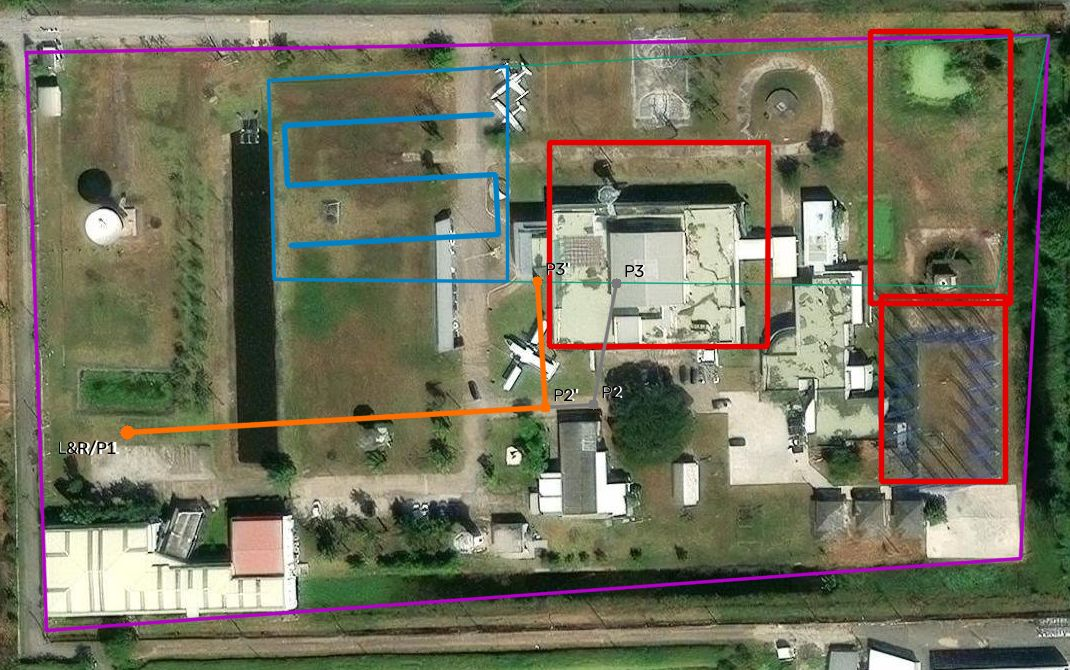
\includegraphics[width=1\textwidth,height=\textheight]{report_figures/field_geometry_2026-08-28.jpg}
\caption{The competition field as briefed on 28 August 2026,
georeferenced against the ground station's cached satellite imagery.
\textbf{Purple} --- the controlled airspace (geofence). \textbf{Teal}
--- the rules' search polygon. \textbf{Blue} --- the three sweep legs
actually flown, over the polygon cut at E 110 m. \textbf{Orange} --- the
briefed transit corridor L\&R/P1 → P2′ → P3′. \textbf{Grey} --- the
corridor the PDF specifies (P2, P3), whose north leg ends on the main
building's roof. \textbf{Red} --- the three no-fly bands declared at the
briefing: the main building, the east end of the search area, and the
rules' orange block. Every straight-line move the mission can make stays
west of the building box.}
\end{figure}

\begin{figure}
\centering
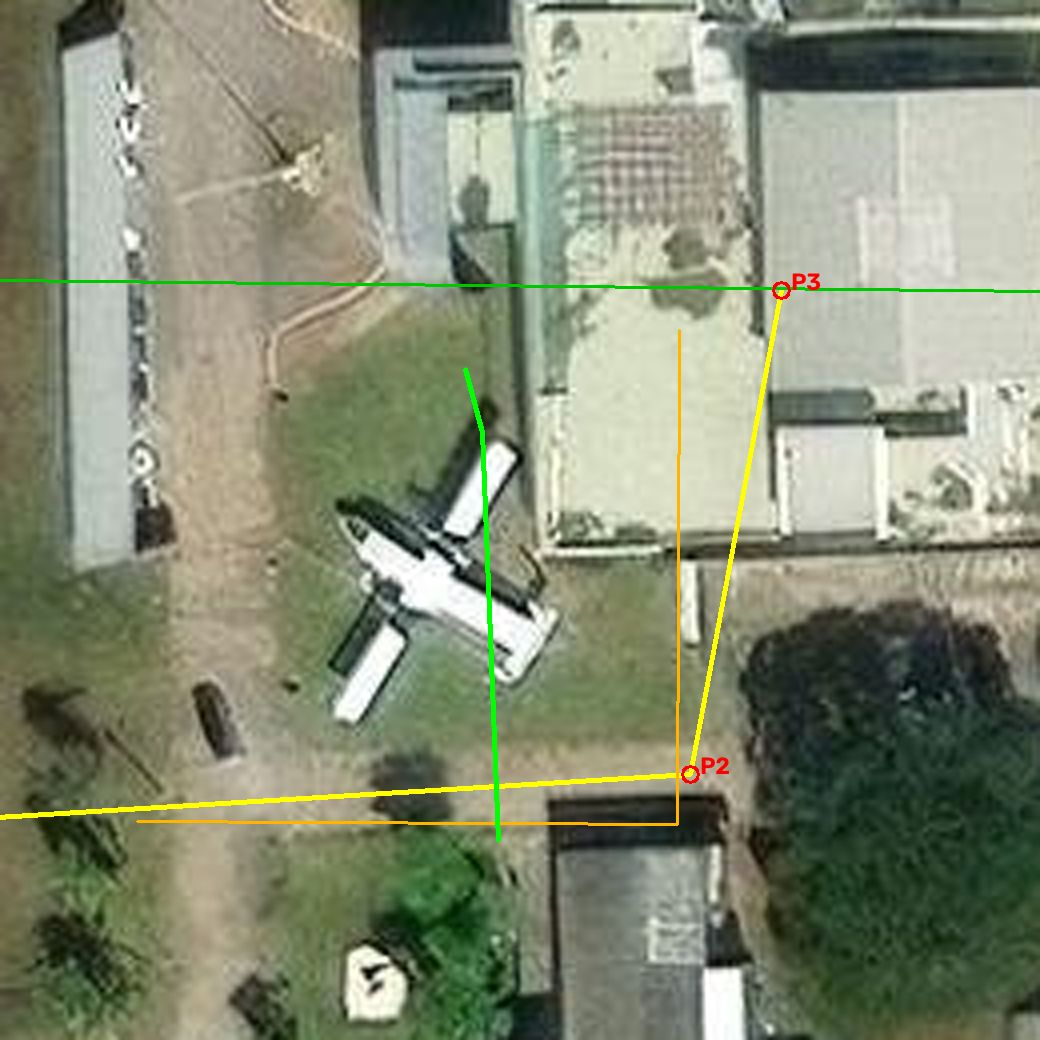
\includegraphics[width=0.62\textwidth,height=\textheight]{report_figures/corridor_georeference_2026-08-28.jpg}
\caption{The corridor region at 4x. \textbf{Yellow} --- the PDF's
P1→P2→P3 with P2 and P3 marked; the leg between them crosses the
building. \textbf{Orange} --- the route drawn on the committee's own
briefing slide. \textbf{Green} --- the operator's traced corridor,
running up the grass strip between the parked display aircraft and the
building's west wall; P2′ and P3′ are taken from this line and are
accurate to \textbf{±5 m}. Committee-published coordinates, if issued,
replace ours.}
\end{figure}

\textbf{Decode geometry drives the sweep plan.} With the
\textbf{measured} 74.2° lens on a 1280 px-wide sensor, the ground swath
is \texttt{2·h·tan(37.1°)} and marker pixels are
\texttt{1280\ ×\ 0.4\ /\ swath}:

\begin{longtable}[]{@{}
  >{\raggedright\arraybackslash}p{(\columnwidth - 8\tabcolsep) * \real{0.1300}}
  >{\raggedright\arraybackslash}p{(\columnwidth - 8\tabcolsep) * \real{0.1000}}
  >{\raggedright\arraybackslash}p{(\columnwidth - 8\tabcolsep) * \real{0.2500}}
  >{\raggedright\arraybackslash}p{(\columnwidth - 8\tabcolsep) * \real{0.2200}}
  >{\raggedright\arraybackslash}p{(\columnwidth - 8\tabcolsep) * \real{0.3000}}@{}}
\toprule\noalign{}
\begin{minipage}[b]{\linewidth}\raggedright
Altitude
\end{minipage} & \begin{minipage}[b]{\linewidth}\raggedright
Swath
\end{minipage} & \begin{minipage}[b]{\linewidth}\raggedright
400 mm marker
\end{minipage} & \begin{minipage}[b]{\linewidth}\raggedright
1 m pad
\end{minipage} & \begin{minipage}[b]{\linewidth}\raggedright
Role
\end{minipage} \\
\midrule\noalign{}
\endhead
\bottomrule\noalign{}
\endlastfoot
20 m (sweep) & 30.3 m & \textbf{16.9 px} --- below the 18 px decode
floor & \textbf{42 px} --- well above the 18 px blob floor &
\textbf{White-pad finder}: 3 legs, 216 m, 87 s over the cut polygon \\
10.5 m (decode visit) & 15.9 m & \textbf{32 px} --- inside the 25--35 px
band proven in flight & 80 px & \textbf{Id reader}: hover and dwell
until the marker decodes (\textasciitilde47 s) \\
12 m (the alternative) & 18.2 m & 28.2 px & 70 px & Would decode in
flight, but 5 legs / 344 m / 142 s and lower clearance over the display
aircraft \\
\end{longtable}

Flying the survey at 20 m and paying for a decode visit only where a
white pad was actually seen is \textbf{55 s cheaper} than sweeping at 12
m on this polygon, and keeps the aircraft above the field obstacles the
committee flagged.

\begin{figure}
\centering
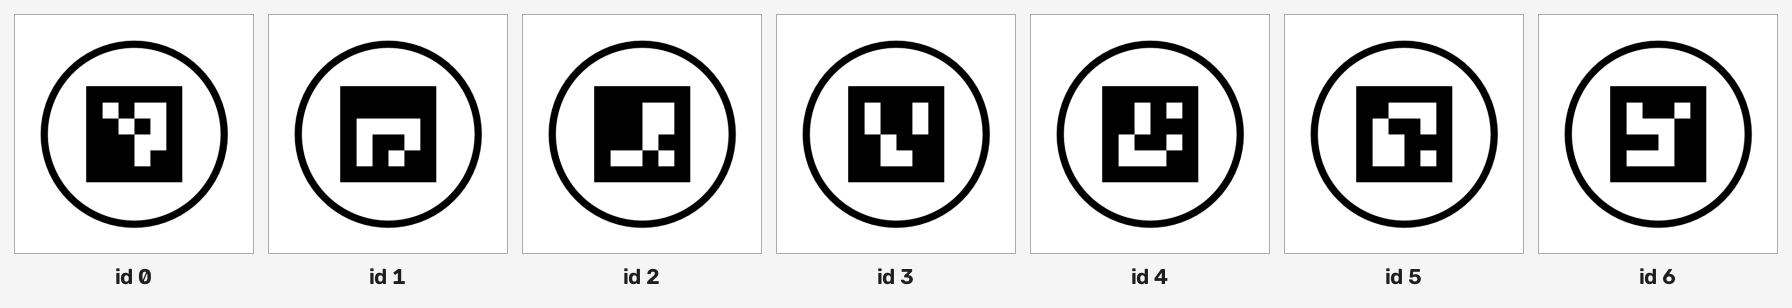
\includegraphics[width=1\textwidth,height=\textheight]{report_figures/pad_faces_ids_0_6.png}
\caption{The seven landing-pad faces the mission must tell apart --- 1 x
1 m white square, 750 mm diameter ring, 400 mm \texttt{DICT\_4X4\_50}
marker. Rendered here by
\texttt{vision.detectors.aruco.render\_pad\_bgr}, the same function that
generates the simulator's pad textures and the detector's test images,
so what the detector is tested against is what the simulator shows. Six
of these are placed on the field and four are assigned to us; \textbf{id
0 is a real pad} --- the rules' Figure 7 encodes 1, 2, 0, 4, 5, 6.}
\end{figure}

\textbf{Window budget drives the mission shape.} A full four-egg flight
is budgeted at \textbf{894 s of the 1200 s window} (17 s take-off + 53 s
ingress + 24 s climb/transition + 87 s sweep + 188 s decode visits + 420
s of four serves + 17 s + 53 s egress + 35 s landing). The last
delivery's gate therefore runs with \textbf{516 s remaining} against a
300 s floor. Carrying all four eggs in one flight --- rather than four
one-egg flights --- is what buys that margin, and the briefing
explicitly permits it.

\hypertarget{selected-delivery-system-configuration-and-architecture}{%
\subsection{2.2 Selected delivery system --- configuration and
architecture}\label{selected-delivery-system-configuration-and-architecture}}

\textbf{Vehicle configuration: single multirotor, hexa-X.} The mission
is a confined urban field with a vertical take-off and landing
requirement, a 1 m landing target, and a fragile payload; a multirotor
is the only sensible class, and six rotors were chosen over four for
three reasons that matter operationally:

\begin{enumerate}
\def\labelenumi{\arabic{enumi}.}
\tightlist
\item
  \textbf{Rotor-out tolerance.} With one motor lost, PX4's
  sequential-desaturation allocator mixes roll, pitch and thrust before
  yaw, so a hexacopter keeps attitude and thrust authority and gives up
  only yaw. That is recoverable by the safety pilot; on a quad it is
  not. (Measured in SITL: unallocated yaw torque rises to 0.25 with the
  allocator still solving for the other axes.)
\item
  \textbf{Payload and mass margin.} Four boxed eggs plus a four-latch
  rack on a 1.0 m frame with 18-inch props hovers at \textasciitilde31
  \% of available thrust, so the motors loaf and retain full authority
  against gusts.
\item
  \textbf{Availability.} The X6100 airframe, ESCs and props were lent
  complete, which converted a procurement risk into flight time.
\end{enumerate}

A single aircraft --- rather than a cooperative search-and-deliver pair
--- keeps mass, cost and failure surface small, and the registry-based
search removes the need for a second vehicle to find pads.

\textbf{System architecture.}

\begin{verbatim}
AIR SEGMENT                                        GROUND SEGMENT
+---------------------------------------+        +-----------------------------+
| Pixhawk 6X (PX4 v1.17)                |        | Safety-pilot RC (ELRS)      |
|   attitude/position control, geofence,|  RC +  |   manual takeover, kill      |
|   FC-level failsafes, RTL             |<------>|                             |
|        ^  MAVLink (serial)            | MAVLink| Web GCS (Svelte + FastAPI)  |
|        |                              | on ONE |   live map, camera, plan,    |
| Raspberry Pi CM4 (companion)          | radio  |   4-of-6 queue editor, GO,   |
|   mission orchestrator (async Python) |        |   confirmed-pad readout, KILL|
|   vision worker (OpenCV ArUco)        |  WiFi  |                             |
|   safety watchdog (2 Hz)              |<------>| (CM4 raises its own local AP |
|   audit trail + frame recorder        |        |  — no internet, no 4G)       |
|        ^                              |        +-----------------------------+
|   OV9281 nadir camera (1280x720 mono, |
|   global shutter, hard-mounted)       |        FPV camera + 5.8 GHz VTX
|   TFmini-S lidar  ·  non-RTK GNSS     |        -> the "transmit" half of the
|   4 egg latches (AUX 4/1/2/3)         |           imaging requirement
+---------------------------------------+
\end{verbatim}

The flight-management stack is a \textbf{non-proprietary, open-source
architecture} (PX4 on Pixhawk 6X) integrated by the team, which complies
with the rules' prohibition on complete proprietary flight packages. All
higher-level autonomy runs on the CM4 as deterministic classical code
that the team wrote.

\textbf{Rationale for the key decisions:}

\begin{itemize}
\tightlist
\item
  \emph{Classical CV, never ML, in the flight loop.} The target is a
  fiducial marker; an OpenCV ArUco decode is deterministic, cheap on a
  CM4, and auditable frame by frame. No torch, no YOLO, no VLM, no
  cloud, no network.
\item
  \emph{Land-ON, then release.} Scoring pays for the egg being placed on
  the pad intact. Releasing from the air risks a broken egg for zero
  payload score, so the release is hard-gated behind a confirmed
  touchdown and is skipped and audited if telemetry says the aircraft is
  airborne.
\item
  \emph{The id is the authority, not the position.} A pad that decodes
  to the wrong id can never steer a descent, and the LAND gate refuses
  to commit unless the assigned id was decoded during the approach.
\item
  \emph{Vision owns the final metre.} Without RTK the GNSS fix wanders
  by more than the pad is wide, so the terminal descent is closed by the
  camera.
\item
  \emph{The GCS monitors; it does not fly.} One operator click per
  flight starts it; everything after that is on board, so a WiFi dropout
  costs a picture, never the mission.
\end{itemize}

\hypertarget{concept-of-operations}{%
\subsection{2.3 Concept of operations}\label{concept-of-operations}}

A \textbf{FLIGHT} is one arm→disarm cycle. A \textbf{DELIVERY} is one
pad served inside a flight, and each delivery is scored independently.
With four eggs aboard, the whole mission is normally \textbf{one flight
containing four deliveries}:

\begin{verbatim}
PREFLIGHT   operator loads the 4 assigned ids as an ordered queue, confirms the
            eggs are racked and the crew is clear -> ONE "GO" click
   -> TAKEOFF        arm, climb out, then close the last metres en route
   -> TRANSIT_INGRESS  P1 -> P2' -> P3' at 20 m        (scored per coordinate)
   -> SEARCH         boustrophedon sweep of the cut search polygon at 20 m,
                     registering every white pad seen; decode visits at 10.5 m
                     read the ids; the sweep stops as soon as every id this
                     flight owes is confirmed
   -> for each assigned id, in turn (one DELIVERY each):
        LOCALIZE     hop to the pad at sweep altitude, descend in verified
                     altitude rungs, re-centring on the decoded marker
        LAND         land ON the pad (final rung tolerance 0.2 m on a 1 m pad)
        DROP         after touchdown confirms + 2 s settle, open that egg's latch
   -> TRANSIT_EGRESS   P3' -> P2' -> P1 at 20 m        (scored per coordinate)
   -> LAND at L&R -> DISARM (resupply crew may approach)
\end{verbatim}

\textbf{Search-and-identify tactic.} A flight whose assigned ids are not
all in the registry flies the sweep. Every pad the camera sees is
clustered by decoded id with a k-vote confirmation, so a single
mis-decode cannot create a target. A pad seen as a white blob but not
decoded is revisited at 10.5 m and the aircraft dwells until the marker
reads; a pad decoded but short of its vote quota gets a cheap vote
top-up visit instead of a re-sweep. The registry persists across
flights, so a later flight whose whole assignment is already registered
flies \textbf{direct}, with no sweep at all.

\textbf{Delivery tactic (land-ON, touchdown-gated).} Over the assigned
pad the aircraft descends through altitude rungs, re-centring on the
decoded marker at each rung with a tightening tolerance down to
\textbf{0.2 m} before the final descent. Three gates protect the egg:

\begin{itemize}
\tightlist
\item
  the \textbf{id-verified LAND gate} refuses to land unless the
  delivery's own assigned id was decoded during the approach --- a
  wrong-id pad or an undecoded blob can never commit the egg;
\item
  the \textbf{centred-final-rung gate} refuses to land if the re-centre
  never converges, climbing back and deferring instead, with one
  re-approach if the window allows;
\item
  the \textbf{touchdown gate} releases only after PX4 reports the
  vehicle landed, plus a 2 s settle; if telemetry reads airborne at the
  release point the release is skipped and audited.
\end{itemize}

Between deliveries inside a flight the aircraft stays \textbf{armed} on
the pad (\texttt{COM\_DISARM\_LAND\ =\ -1}), so no re-arm happens over
the field and PX4's home point stays pinned to the launch site.

\textbf{Repeat-delivery and resupply tactic.} Between flights the
aircraft lands at L\&R and disarms so the crew can approach. The
20-minute window clock starts at the \textbf{first} GO. A per-flight
gate refuses a launch that cannot finish inside the window unless the
operator explicitly accepts the overtime penalty, and a
\textbf{per-delivery gate} re-checks time and battery before
\textbf{every} egg: failing it skips the remaining eggs of that flight
and brings them home rather than starting a descent the budget cannot
finish.

\textbf{Planned battery egress --- the mission gives up eggs, not the
aircraft.} Below \textbf{30 \%} indicated the flight starts nothing new:
the sweep stops, decode visits are skipped, the delivery gate refuses,
and the aircraft flies the \textbf{normal egress through the corridor},
lands and disarms. The crew swaps to the second pack and the
\textbf{recovery flight} serves what is still owed --- flying direct off
the registry, and firing only the latches that still hold eggs (the crew
does not re-rack eggs at a battery swap, so the recovery flight
continues the wiring order through the unfired holds). The 15 \%
return-to-home and 10 \% land-in-place thresholds sit
\textbf{underneath} this as failsafes; the point of the planned egress
is never to reach them.

\begin{center}\rule{0.5\linewidth}{0.5pt}\end{center}

\hypertarget{engineering-design-analysis-40-pts}{%
\section{3. Engineering Design \& Analysis (40
pts)}\label{engineering-design-analysis-40-pts}}

\hypertarget{airframe-structure-and-integrity}{%
\subsection{3.1 Airframe structure and
integrity}\label{airframe-structure-and-integrity}}

\begin{itemize}
\tightlist
\item
  \textbf{Frame:} \textbf{EFT X6100} hexa-X, \textbf{1.000 m wheelbase}
  (0.500 m arm radius), folding carbon arms and carbon plates, frame
  mass \textasciitilde2.75 kg, manufacturer MTOW \textasciitilde12 kg.
  Provided by DRON.
\item
  \textbf{Rotor clearance:} adjacent motors sit 500 mm apart on the
  hexagon; with \textbf{18 × 6.5 in} propellers (457 mm diameter) the
  tip-to-tip gap is \textbf{\textasciitilde43 mm}, so there is no rotor
  overlap and no interaction between discs (DCOS ``clearance between
  moving parts'').
\item
  \textbf{Payload rack:} four independent holds arranged front-left,
  front-right, rear-left and rear-right about the centre of gravity,
  each sized to accept the organiser's heart-shaped box
  (\textasciitilde16 × 7 × 18 cm, 300-gsm) rather than a bare egg. The
  release order is \textbf{diagonal} so the net CG moment is zero when
  full and zero again after the first two eggs leave.
\item
  \textbf{Ground clearance:} the camera and the lidar are carried 0.25 m
  below the CG on the underside; the landing gear keeps both, and the
  loaded boxes, clear of the pad at touchdown.
\item
  \textbf{Structural load cases:} flight manoeuvre load is
  envelope-limited to \textbf{30° tilt} (\texttt{MPC\_TILTMAX\_AIR}) and
  \textbf{2 m/s² horizontal acceleration} (\texttt{MPC\_ACC\_HOR}); the
  land-ON touchdown is absorbed at \textbf{\texttt{MPC\_LAND\_SPEED} =
  0.3 m/s} with the final autonomous descent pinned to \textbf{0.4 m/s}
  (\texttt{MPC\_Z\_V\_AUTO\_DN}); ground handling and transport use the
  folded arms.
\item
  \textbf{Power path:} the \textbf{motors are fed from a separate
  distribution board that the flight controller cannot sense}. A Holybro
  \textbf{PM02D} supplies the Pixhawk 6X and avionics only, and the CM4
  runs from its own power-bank rail so companion current cannot brown
  out the flight controller. This split is deliberate and has one
  important consequence, carried through §3.2: \textbf{any current the
  FC reports is avionics draw, never flight current}, so the battery
  gauge must never be current-fused.
\item
  \textbf{Mass, as weighed 19 August 2026:} \textbf{7.2 kg all-up, ready
  to fly}, with one 17,000 mAh pack (1.5 kg) and four boxed eggs aboard
  --- \textbf{29 \% of the 25 kg rules limit}. Rule adopted after three
  conflicting weighings in one afternoon: \emph{never record a mass
  without recording what was on the aircraft} (pack count, power module,
  companion, eggs).
\item
  \textbf{Open items (honest status):} a formal \textbf{CG placement
  record} and a \textbf{quantified structural load-factor margin} are
  not documented; the aircraft is trimmed by flight behaviour, not by a
  calculated CG envelope. The organiser's boxes are heavier than the 50
  g dummies in the weighed figure, so the aircraft is re-weighed with
  the real cargo at the field committee's scale.
\end{itemize}

\hypertarget{propulsion-and-flight-performance-analysis}{%
\subsection{3.2 Propulsion and flight-performance
analysis}\label{propulsion-and-flight-performance-analysis}}

\begin{longtable}[]{@{}
  >{\raggedright\arraybackslash}p{(\columnwidth - 4\tabcolsep) * \real{0.3600}}
  >{\raggedright\arraybackslash}p{(\columnwidth - 4\tabcolsep) * \real{0.4200}}
  >{\raggedright\arraybackslash}p{(\columnwidth - 4\tabcolsep) * \real{0.2200}}@{}}
\toprule\noalign{}
\begin{minipage}[b]{\linewidth}\raggedright
Parameter
\end{minipage} & \begin{minipage}[b]{\linewidth}\raggedright
Value
\end{minipage} & \begin{minipage}[b]{\linewidth}\raggedright
Basis
\end{minipage} \\
\midrule\noalign{}
\endhead
\bottomrule\noalign{}
\endlastfoot
Airframe & EFT X6100 hexa-X, 1.000 m wheelbase, 18 × 6.5 in props & as
built \\
Motors & \textbf{6 × EFT E5 5008, 335 KV} & as built \\
ESC & 6 × PWM-only ESC (\textbf{no telemetry lead} --- see §3.3) & as
built \\
Max thrust per motor & \textbf{37.65 N} (3,838 gf at 100 \% throttle, 24
V, 18 × 6.5 in) & manufacturer bench table (Power-System-Guide) \\
Max thrust, 6 rotors & \textbf{226 N ≈ 23 kgf} & 6 × above \\
All-up weight (flight-ready, 4 boxed eggs) & \textbf{7.2 kg} & weighed
2026-08-19 \\
Thrust-to-weight & \textbf{≈ 3.2 : 1} & 23 kgf / 7.2 kg \\
Hover thrust fraction & \textbf{≈ 31 \%} of maximum (11.8 N per motor) &
as above \\
Hover current & \textbf{≈ 30 A} at 6S (\textasciitilde670 W) & E5 bench
anchor scaled by mass\^{}1.5 \\
Hover throttle, measured in flight & \textbf{0.59--0.64} & ULog,
2026-08-27 \\
Battery (mission) & \textbf{6S 17,000 mAh semi-solid}, 10 C, 1.5 kg,
25.1 V full (4.18 V/cell), \textasciitilde22.6 V empty (3.77 V/cell) &
as fitted 2026-08-19 \\
Battery (spare, for the swap) & 6S 15,000 mAh & as held \\
Usable energy & \textbf{12,750 mAh} (75 \% of nameplate) & policy \\
Planned cost of a four-delivery flight & \textbf{4,700 mAh} (1,750 first
delivery + 3 × 900 + 250 margin) & \texttt{battery:} seeds, deliberately
conservative \\
Cruise / sweep speed & 3.0 m/s (\texttt{MPC\_XY\_CRUISE}), max 5.0 m/s
(\texttt{MPC\_XY\_VEL\_MAX}) & config \\
Climb / take-off & 1.5 m/s (\texttt{MPC\_Z\_VEL\_MAX\_UP},
\texttt{MPC\_TKO\_SPEED}) & config \\
Autonomous descent / touchdown & 0.4 m/s (\texttt{MPC\_Z\_V\_AUTO\_DN})
/ 0.3 m/s (\texttt{MPC\_LAND\_SPEED}) & config \\
Auto yaw rate & 25 °/s (\texttt{MPC\_YAWRAUTO\_MAX}) & config \\
\end{longtable}

\textbf{Excess-thrust margin (DCOS).} Hovering at \textasciitilde31 \%
of available thrust leaves roughly a two-thirds throttle headroom, so
the motors run cool, the allocator never saturates (confirmed in the 27
August logs), and full control authority remains for gust rejection. The
margin holds across the loaded and empty cases because four boxed eggs
are a small fraction of a 7.2 kg aircraft.

\textbf{Energy --- the binding constraint, stated plainly.} On paper the
budget is comfortable: 4,700 mAh planned against 12,750 mAh usable. In
flight it is not that simple, because this aircraft \textbf{cannot
measure current}. With \texttt{BAT1\_CAPACITY\ =\ -1} the state of
charge is derived from voltage alone, and PX4 only load-compensates when
it has a current reading --- which it does not --- so the indicated
percentage sags under thrust and rebounds when the aircraft settles.
Measured across four flights on 27 August:

\begin{longtable}[]{@{}
  >{\raggedright\arraybackslash}p{(\columnwidth - 2\tabcolsep) * \real{0.7200}}
  >{\raggedright\arraybackslash}p{(\columnwidth - 2\tabcolsep) * \real{0.2800}}@{}}
\toprule\noalign{}
\begin{minipage}[b]{\linewidth}\raggedright
Observation
\end{minipage} & \begin{minipage}[b]{\linewidth}\raggedright
Value
\end{minipage} \\
\midrule\noalign{}
\endhead
\bottomrule\noalign{}
\endlastfoot
Continuous sweep flight, full pack & 93 \% → 26 \% indicated in
\textbf{5.8 min} \\
Three flights with pauses, full pack & 96 \% → 25 \% indicated over
\textbf{8.6 min} of flying \\
Indicated drain under load & \textbf{\textasciitilde7--8 percentage
points per minute} \\
Extrapolated time to the 15 \% return floor & \textbf{minute 8.5--10} of
powered flight \\
KMITL plan & \textbf{894 s budgeted}, \textasciitilde10--13 min
realistic \\
Cell voltage at 25 \% indicated, rested & 3.87--3.92 V/cell ⇒ true state
of charge \textasciitilde55--65 \% \\
\end{longtable}

The gauge is therefore \textbf{pessimistic} --- the pack almost
certainly holds the energy (roughly 10 Ah of 17 Ah for a 15-minute
flight at \textasciitilde40 A) --- but the \textbf{true capacity has
never been measured}, so the flight is planned against the gauge, not
against the optimistic interpretation. Consequences, all already
implemented: the per-delivery gate gives up eggs 3 and 4 safely rather
than the aircraft; the planned 30 \% egress flies the scored corridor
home instead of falling into a straight-line failsafe RTL; and a
\textbf{second charged pack with an automatic recovery flight} is the
primary mitigation. The one measurement that closes the question is the
\textbf{mAh returned by the charger} after a flight, which is recorded
from now on. The battery percentage floors were \textbf{not} lowered
further: the ESCs' low-voltage cut-off is unknown, and a floor is worth
more than an egg.

\textbf{Flight-performance verification against §2.1.} Requirements met:
the survey covers the cut polygon in 3 legs at 3 m/s; transit holds 20 m
in the barometric frame (commanded 19.5 m --- see §3.3 --- measured
maximum 19.69 m in the four-egg SITL run, no ceiling flag); and a
complete real mission --- transit, survey, two land-ONs with releases,
egress and landing 0.7 m from the launch point --- was flown in
\textbf{4 min 12 s} on 27 August.

\hypertarget{avionics-and-sensor-subsystem}{%
\subsection{3.3 Avionics and sensor
subsystem}\label{avionics-and-sensor-subsystem}}

\begin{longtable}[]{@{}
  >{\raggedright\arraybackslash}p{(\columnwidth - 4\tabcolsep) * \real{0.1600}}
  >{\raggedright\arraybackslash}p{(\columnwidth - 4\tabcolsep) * \real{0.2800}}
  >{\raggedright\arraybackslash}p{(\columnwidth - 4\tabcolsep) * \real{0.5600}}@{}}
\toprule\noalign{}
\begin{minipage}[b]{\linewidth}\raggedright
Subsystem
\end{minipage} & \begin{minipage}[b]{\linewidth}\raggedright
Component
\end{minipage} & \begin{minipage}[b]{\linewidth}\raggedright
Function and status
\end{minipage} \\
\midrule\noalign{}
\endhead
\bottomrule\noalign{}
\endlastfoot
Flight controller & \textbf{Holybro Pixhawk 6X}, PX4 \textbf{v1.17.0} &
\texttt{SYS\_AUTOSTART\ =\ 6001} (generic hexarotor X),
\texttt{CA\_ROTOR\_COUNT\ =\ 6},
\texttt{PWM\_MAIN\_FUNC1..6\ =\ 101..106} --- verified pin by pin with
\texttt{ACTUATOR\_TEST}, all six motors observed spinning in the correct
order and direction \\
Companion computer & \textbf{Raspberry Pi CM4} & Mission orchestrator,
vision, watchdog, GCS server; own power rail \\
Nadir camera & \textbf{Meige OV9281} USB UVC, 1280 × 720 \textbf{mono
global shutter} & Sole control-authority sensor: ArUco decode +
white-pad cue. \textbf{FOV measured 74.2°} (fx ≈ 847 px).
\textbf{Hard-mounted, no gimbal.} \\
Camera orientation & \textbf{Mount yaw measured 180°} & The camera is
bolted \textbf{upside down}; image row 0 looks at the tail. Measured
from four independent placements of a floor target around the levelled
airframe (180.3 / 187.4 / 183.4 / 186.1°, snapped to the bolted 180) \\
Height (primary) & \textbf{Barometer}, \texttt{EKF2\_HGT\_REF\ =\ 0} &
GPS height reference was measured diverging \textbf{10.8 m peak-to-peak}
inside one flight and returned an aircraft that was tracking transit
correctly --- the barometer is the reference at both fields \\
Height (terminal) & \textbf{Benewake TFmini-S} downward lidar, TELEM3
(\texttt{SENS\_TFMINI\_CFG\ =\ 103}) & \texttt{EKF2\_RNG\_CTRL\ =\ 1},
conditional aiding below \texttt{EKF2\_RNG\_A\_HMAX\ =\ 7.0} m --- pins
the final metres of the descent \\
Optical flow & \textbf{None} (\texttt{EKF2\_OF\_CTRL\ =\ 0}) & No flow
module in the kit; the decision is pinned so it cannot silently
re-enable \\
GNSS & Non-RTK GPS/compass & Measured 14--16 satellites, horizontal
accuracy ≤ 2 m at the practice field \\
Power sensing & Holybro \textbf{PM02D}, avionics only &
\texttt{BAT1\_CAPACITY\ =\ -1} forces the \textbf{voltage-only} gauge;
\texttt{BAT1\_V\_DIV} closed by multimeter (24.9 V at the connector vs
24.89 V reported --- 0.04 \%) \\
ESC telemetry & \textbf{None --- physically absent} & The ESCs are
PWM-only with no telemetry lead; \texttt{DSHOT\_TEL\_CFG\ =\ 0} and zero
\texttt{ESC\_STATUS} even after the FC accepted a message-interval
request. Per-motor current is the only signal a motor-out detector could
use, so both detector layers were \textbf{deleted rather than left
inert}; the safety pilot is the mitigation, and restoring the feature
starts with buying telemetry-capable ESCs \\
Imaging downlink & FPV camera + 5.8 GHz VTX & The ``transmit'' half of
the imaging rule, independent of WiFi \\
\end{longtable}

\textbf{Why the camera pose is load-bearing.} With no gimbal the camera
pitches with the body, so \texttt{vision/projection.py} composes roll
and pitch into every pixel→ground fix; a translating multirotor holds
10--15° of tilt, which uncompensated is \textasciitilde2 m of error at
12 m altitude. Both the mount yaw and the lens FOV had shipped as
\textbf{assumptions} and both were wrong --- the yaw by
\textasciitilde180°, which point-mirrored every fix about the aircraft
and is exactly the signature of a sweep that sees pads and never
re-acquires them. They are now bench measurements, and the simulator
carries the same 180° mount so the same error would fail in simulation
instead of at the field.

\textbf{Exposure --- the fix that made in-flight decoding work.} The
camera's own auto-exposure meters the whole frame, which at this field
is sunlit grass at \textasciitilde130 counts; a white pad is four to
five times that albedo and clips at 255, and the marker's black modules
bleed into 1--3 px lines. That is why 2,788 frames of one flight decoded
nothing with a pad plainly in view. The grabber now runs a
\textbf{highlight-priority auto-exposure}: it meters the brightest 0.2
\% of the frame every 0.5 s and steps the manual exposure to hold that
between \textbf{190 and 225}, caps the ground mean at 55 when nothing
bright is in view, and never exceeds a 4 ms exposure (about 1.3 px of
smear at 3 m/s from 8 m). A marker carried at running speed across 8--10
m decoded \textbf{56--65 \% of frames} at 25--35 px on the bench --- the
sweep's own pixel size at twice its angular rate --- and the 26 August
flight decoded ids in the air for the first time.

\begin{figure}
\centering
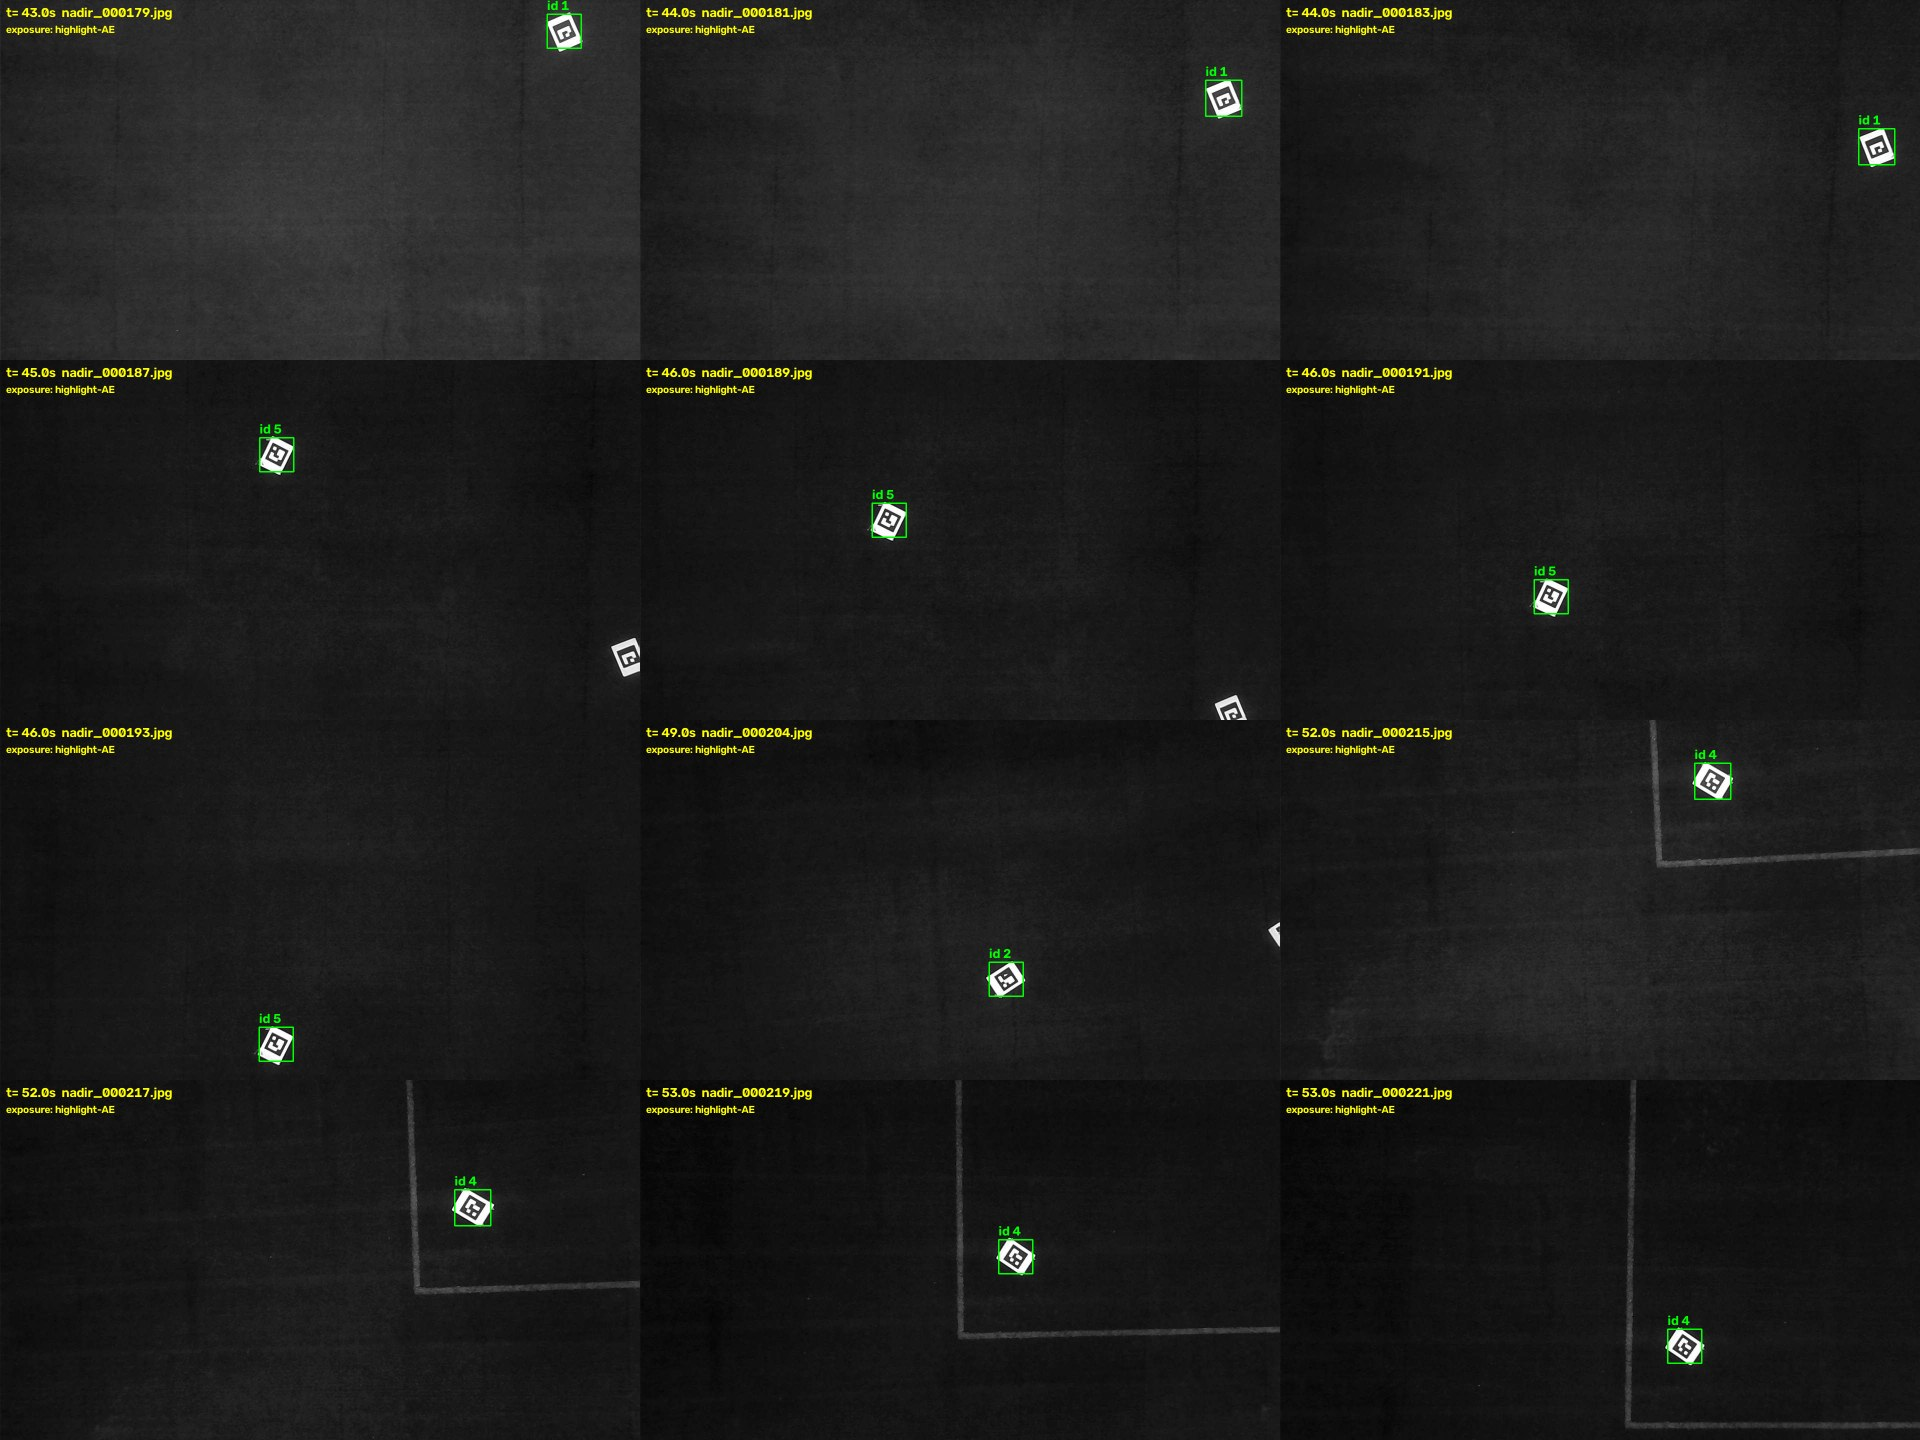
\includegraphics[width=1\textwidth,height=\textheight]{report_figures/decode_real_flight_2026-08-26.jpg}
\caption{Real flight, 26 August 2026: twelve nadir frames in which the
detector decoded a pad \textbf{in the air}, with the marker outlined and
the id it read. Markers 1, 5, 2 and 4 appear here. Every frame is
labelled \texttt{exposure:\ highlight-AE} --- this is the flight
immediately after the exposure fix, on the same camera and the same
field that had produced 2,788 frames and zero decodes two flights
earlier.}
\end{figure}

\hypertarget{software-system-architecture-operating-modes-and-safety-features}{%
\subsection{3.4 Software system architecture --- operating modes and
safety
features}\label{software-system-architecture-operating-modes-and-safety-features}}

The autonomy stack is a \textbf{deterministic, offline, classical}
system on the CM4 (Python 3.12, async throughout, MAVSDK to the flight
controller). There is no LLM, no cloud and no network in flight ---
network use is an automatic disqualification. Layers:

\begin{itemize}
\tightlist
\item
  \textbf{Mission orchestrator} --- the state machine of §2.3; one
  long-running process flies every flight of the window, holding in
  PREFLIGHT before each.
\item
  \textbf{Live plan builder} --- rebuilds the plan per flight and
  re-renders it at every gate release and every serve, so the ground
  station always shows what the aircraft is actually going to do next.
\item
  \textbf{Vision worker} --- ArUco decode plus the white-pad blob cue,
  with a frame-age gate and multi-pad fixes per frame.
\item
  \textbf{Pad registry} --- id-keyed clusters with k-vote confirmation,
  median-fused geolocation, and a maximum fix distance so a wild
  projection cannot create a target.
\item
  \textbf{Terminal controller} --- the rung descent, the id-verified
  LAND gate, the centred-final-rung gate and the touchdown-gated
  release.
\item
  \textbf{Safety watchdog} --- a 2 Hz phase-aware monitor (below).
\item
  \textbf{Time and energy policies} --- the window reserve, the
  per-flight and per-delivery gates, and the pack budget with swap
  detection.
\item
  \textbf{Audit trail and verifier} --- every flight writes a
  machine-readable \texttt{audit.jsonl} (1 Hz telemetry samples, transit
  pass/miss per point per direction, flight and delivery
  start/release/end lines); a \textbf{fail-closed} post-flight verifier
  re-scores the flight against it.
\item
  \textbf{Ground station} --- a Svelte + FastAPI web GCS: live map with
  the corridor drawn, camera view, the live plan, the ordered 4-of-6
  mission-queue editor, the per-flight GO, an emergency KILL, and a
  confirmed-pad readout that shows \textbf{each pad id as the ArUco
  glyph itself} so the operator matches the committee's card
  picture-to-picture instead of translating it to a number.
\end{itemize}

\textbf{Operating modes:} PREFLIGHT · TAKEOFF · TRANSIT\_INGRESS ·
SEARCH · LOCALIZE · LAND · DROP · TRANSIT\_EGRESS · RTH · ABORT.

\textbf{Companion-side watchdog (2 Hz, phase-aware).} Every check below
is active in flight; none can be switched off:

\begin{longtable}[]{@{}
  >{\raggedright\arraybackslash}p{(\columnwidth - 2\tabcolsep) * \real{0.4500}}
  >{\raggedright\arraybackslash}p{(\columnwidth - 2\tabcolsep) * \real{0.5500}}@{}}
\toprule\noalign{}
\begin{minipage}[b]{\linewidth}\raggedright
Condition
\end{minipage} & \begin{minipage}[b]{\linewidth}\raggedright
Response
\end{minipage} \\
\midrule\noalign{}
\endhead
\bottomrule\noalign{}
\endlastfoot
Geofence breach & Return to home (proximity inside the margin =
warning) \\
No-fly-zone entry & Return to home \\
Altitude ceiling & Warning above \textbf{30.5 m}; sustained above
\textbf{31.5 m} → return to home \\
Below the 10 m search floor outside the delivery descent & Advisory
anomaly \\
Terrain proximity / unknown terrain (lidar) & Advisory, escalating to
return to home \\
Battery below \textbf{30 \%} (planned) & Stop starting anything new; fly
the corridor egress home, land, disarm \\
Battery below \textbf{15 \%} / \textbf{10 \%} & Return to home / land in
place \\
Battery telemetry NaN, sustained & Loud operator anomaly --- never a
silent loss of battery protection \\
GPS 3D-fix loss, debounced 5 s & Return to home \\
Datalink loss, debounced 5 s & Return to home \\
Telemetry stale \textgreater{} 10 s & Return to home \\
Camera frame older than 2 s & Treated as \textbf{no detection} --- a
frozen image can never satisfy the LAND gate \\
Time budget exhausted & Return to home \\
\textbf{Pilot takeover} (manual mode from the RC) & Orchestrator
\textbf{stands down}; no companion command may fight the pilot \\
\textbf{FC-commanded RTL or LAND} we did not ask for & Orchestrator
\textbf{stands down} (\texttt{FC\ FAILSAFE}) on the first tick \\
\end{longtable}

The last two are recent and were both bought with real flights. On 26
August PX4's own vertical fence returned an aircraft that was flying
correctly, and the mission never noticed: it kept sweeping, and its next
waypoint went out while the RTL was 0.46 m from touchdown --- PX4 obeyed
and climbed back out. The watchdog now records which AUTO mode \emph{we}
commanded and treats any other FC-initiated RTL or LAND as a stand-down.
On 27 August the first version of that rule fired on \textbf{our own}
landing 0.3 s after the first real egg was released, so two further
rules were added: a LAND while on the ground is never a failsafe, and an
expectation is \textbf{consumed} when the flight controller leaves the
mode by itself, never cleared ahead of time by the next command.

\textbf{Flight-controller-level failsafes} (these fire even if the
companion dies; all are written at mission start and read back):

\begin{itemize}
\tightlist
\item
  \texttt{NAV\_DLL\_ACT} = Return (datalink loss) ·
  \texttt{NAV\_RCL\_ACT} = Return (RC loss, with
  \texttt{COM\_RCL\_EXCEPT} so an autonomous no-RC flight is not
  spuriously returned) · \texttt{GF\_ACTION} = \textbf{3, Return}.
\item
  Battery: \texttt{BAT\_LOW\_THR} 25 \% · \texttt{BAT\_CRIT\_THR} 15 \%
  · \texttt{BAT\_EMERGEN\_THR} 7 \% with \texttt{COM\_LOW\_BAT\_ACT} =
  3, arranged so the FC's critical threshold coincides with the
  companion's return-home floor and its emergency threshold sits under
  the companion's land floor --- the two layers never race.
\item
  \texttt{RTL\_RETURN\_ALT} = \textbf{25 m}: any failsafe RTL is a
  straight line home over the building, the display aircraft and the
  tree line, and 25 m clears them while leaving 5 m under the ceiling
  for PX4's in-flight home-altitude drift. PX4's 60 m default would bust
  the ceiling.
\item
  \texttt{GF\_MAX\_VER\_DIST} = 50 m as a gross-runaway net only: the
  FC's vertical fence is home-relative, and PX4 1.17 rewrites the home
  altitude in flight, so it cannot be trusted to hold the rules'
  ceiling. The ceiling is enforced by the companion against a latched
  home altitude.
\end{itemize}

\textbf{Three defects found in flight and fixed --- worth stating
because they are the reason the numbers in this report can be trusted:}

\begin{enumerate}
\def\labelenumi{\arabic{enumi}.}
\tightlist
\item
  \textbf{The mission clock ran at 1/20 speed on the real aircraft} (26
  August). Mission time is read from the vehicle's own clock, and a
  re-fed identical timestamp was resetting the wall-clock anchor, so
  every deadline --- the 20-minute window, the delivery gates, the
  leg-progress guard, the touchdown timeouts --- stretched twentyfold
  and none of them could have fired at KMITL. Flight time is now
  accumulated per epoch as \texttt{min(vehicle,\ wall)} and a re-fed
  sample moves nothing.
\item
  \textbf{PX4 rewrites \texttt{home.alt} in flight} (upstream issue in
  1.17), which moves the reported relative altitude while the aircraft
  physically holds station: measured shifts of +3.29 / −4.65 / +0.91 /
  +1.17 / −3.18 m across five flights, and one of them returned a
  correctly-flying aircraft through the ceiling watchdog. The height
  used by the mission is now
  \texttt{altitude\ −\ home\ altitude\ latched\ at\ arming}, and home
  updates are refused once airborne.
\item
  \textbf{The geofence action had been ``Hold'', not ``Return'', for its
  whole life} --- the setter wrote the wrong enum value while its own
  name, comment and error text said RTL. The breach response was
  therefore ``stop and loiter outside the fence''. The lesson kept in
  the code: a read-back gate proves a value was stored, never that the
  value means what the caller thinks.
\end{enumerate}

\textbf{Software integrity evidence.} \textbf{771 automated tests}
import the real modules --- the mission loop, the terminal controller,
the watchdog, the detector, the projection maths, the flight clock, the
home latch --- and all pass, with linting and static type-checking
clean. Behavioural changes are test-driven; the SITL gate exercises the
whole sequence end to end; and every real flight is re-scored afterwards
by the fail-closed verifier.

\hypertarget{payload-handling-mechanism}{%
\subsection{3.5 Payload handling
mechanism}\label{payload-handling-mechanism}}

Four independent latches carry four boxed eggs. Each is a metal-gear
servo on a Pixhawk \textbf{AUX} output configured as a peripheral
actuator (\texttt{PWM\_AUX\_FUNC\ n\ =\ 300\ +\ n}), commanded with
\textbf{\texttt{MAV\_CMD\_DO\_SET\_ACTUATOR} (187)} --- PX4 has
\textbf{no handler for \texttt{DO\_SET\_SERVO}}, so that command is
never used. PWM \textbf{1900 µs = release}, \textbf{1100 µs = hold}; one
latch needs \texttt{PWM\_AUX\_MAX\ =\ 2100} to reach its release angle.

\begin{longtable}[]{@{}
  >{\raggedright\arraybackslash}p{(\columnwidth - 4\tabcolsep) * \real{0.4000}}
  >{\raggedright\arraybackslash}p{(\columnwidth - 4\tabcolsep) * \real{0.3000}}
  >{\raggedright\arraybackslash}p{(\columnwidth - 4\tabcolsep) * \real{0.3000}}@{}}
\toprule\noalign{}
\begin{minipage}[b]{\linewidth}\raggedright
\texttt{payload\_id} (release order)
\end{minipage} & \begin{minipage}[b]{\linewidth}\raggedright
Rack position
\end{minipage} & \begin{minipage}[b]{\linewidth}\raggedright
AUX pin / actuator set
\end{minipage} \\
\midrule\noalign{}
\endhead
\bottomrule\noalign{}
\endlastfoot
0 & Front-left & \textbf{4} \\
1 & Rear-right & \textbf{1} \\
2 & Front-right & \textbf{2} \\
3 & Rear-left & \textbf{3} \\
\end{longtable}

The wiring was verified \textbf{pin by pin on the aircraft} with
\texttt{ACTUATOR\_TEST} while disarmed, watching which corner moved ---
the paper table written before that test had the order wrong. The same
session found the four AUX outputs sitting on \textbf{RC passthrough}
functions, i.e.~two egg latches wired to the roll and yaw sticks, which
would have released eggs whenever the aircraft banked.

Safety properties of the release path:

\begin{itemize}
\tightlist
\item
  \textbf{Never airborne.} The release runs only after the flight
  controller reports a landing, plus a 2 s settle. If telemetry reads
  airborne the release is skipped and audited.
\item
  \textbf{Never twice.} Releases are idempotent against a ledger keyed
  by the \textbf{mission-global delivery index}, so two deliveries
  inside one flight can never collide and a retry cannot double-fire.
\item
  \textbf{Never the wrong hold on a recovery flight.} The crew does not
  re-rack eggs at a battery swap, so a recovery flight continues the
  wiring-order progression through the latches that \textbf{still hold
  an egg}, rather than restarting at slot 0 and firing two empty holds.
\item
  \textbf{Manual release is gated too.} The ground station's manual DROP
  is refused while telemetry reads airborne unless the operator
  explicitly forces it.
\end{itemize}

Per DCOS the payload is securely retained in flight and the mechanism
has no unsafe state: a latch failure leaves an egg aboard, which costs a
delivery and nothing else. The rules' prohibitions on simultaneous
multi-cargo release and on winching are both respected --- eggs are
released one at a time, on the ground, one per landing.

\hypertarget{communication-system}{%
\subsection{3.6 Communication system}\label{communication-system}}

\begin{itemize}
\tightlist
\item
  \textbf{RC and telemetry on one link:} a \textbf{RadioMaster NOMAD}
  dual-band system carries both the safety pilot's ELRS control link and
  the MAVLink telemetry the ground station reads (receiver: DBR4
  diversity). This replaced a telemetry radio that failed at the field,
  and it means the GCS panels are fed by the radio rather than by WiFi
  --- a WiFi dropout never freezes the display.
\item
  \textbf{Imagery:} an FPV camera on its own 5.8 GHz VTX satisfies the
  ``transmit'' half of the rules' imaging requirement, and the on-board
  frame recorder satisfies ``record'' by writing a JPEG trail to the
  CM4's own disk. Neither half depends on the WiFi link, so the live
  dashboard image is a debug convenience that can be switched off on
  competition day at no cost.
\item
  \textbf{Frequencies:} ELRS/NOMAD and the VTX operate inside the
  recommended 920--925 / 2400--2500 / 5725--5850 MHz bands. \textbf{No
  4G/LTE, no SIM, no internet} --- their use is a disqualification, and
  the field network is the CM4's own local access point.
\item
  \textbf{On-board routing:} a MAVLink router fans the flight link to
  the orchestrator, the ground station, and an optional QGroundControl
  endpoint that \textbf{defaults to loopback}, so the armed aircraft's
  control plane is never exposed unauthenticated on a field network.
\item
  \textbf{Standby-area discipline (procedural).} The rules forbid
  activating radio control and telemetry while in the standby area, and
  this aircraft raises its own access point at boot. The procedure is
  therefore: \textbf{do not connect the battery until the launch point},
  and keep the ground console closed while waiting.
\end{itemize}

\hypertarget{operating-procedures-normal-and-emergency}{%
\subsection{3.7 Operating procedures (normal and
emergency)}\label{operating-procedures-normal-and-emergency}}

\textbf{Before the field day.} A parameter tool reads back the flight
controller's own state and splits it into a \textbf{STOP block} --- the
values that live on the board and must be correct before flying
(airframe, motor map, battery gauge endpoints, height reference, sensor
ports, fence) --- and an informational block of values the orchestrator
pins at mission start. This exists because the motor map was once found
reading zero, i.e.~the aircraft was unflyable and looked normal; the
cause was never identified, so it is treated as a regression that can
recur and is re-read every field day rather than trusted.

\textbf{Normal operation.} The operator enters the committee's four
assigned ids once, as an ordered queue, using the ArUco glyphs shown on
screen. Then, per flight: the readiness board goes green (link,
arm-ready, EKF, home, sensors, GPS fix, battery ≥ 25 \% resting,
on-ground, geofence, fresh camera frame) → the operator confirms the
eggs are racked and the crew is clear → \textbf{one GO click} → the
aircraft flies the whole flight autonomously → it lands and disarms at
L\&R. The window clock starts at the first GO; the gates manage the
schedule and refuse a launch that cannot finish, unless the operator
explicitly accepts the overtime penalty.

\textbf{Battery swap and recovery flight.} If the planned 30 \% egress
fires, the aircraft comes home through the scored corridor and disarms.
The crew swaps to the second charged pack; the between-flights gate
waits as long as the swap takes. The next GO launches a \textbf{recovery
flight} which flies direct to the pads still owed --- they are already
in the registry --- and fires only the latches that still hold eggs.

\textbf{Emergency operation.} The safety pilot can take manual control
at any instant, and the orchestrator stands down the moment it detects
the takeover. The ground station's KILL cuts motors, guarded by an armed
command session so that an accidental click cannot fire it. Automatic
failsafes --- the companion watchdog and the FC-level RTL on geofence,
datalink, RC and battery --- recover the aircraft without operator
action. On any unhandled mission error the orchestrator commands an
emergency return and land, and the FC failsafe sits underneath that.
Retries within the window are free under the rules, and the mission's
own registry makes a restart cheap: the pads are already known.

\textbf{Brief for the safety pilot.} A commanded mode change may need to
be repeated once: the orchestrator stands down on the first tick, but a
command already in the MAVLink pipeline (\textasciitilde0.5 s) can still
reach the aircraft.

\hypertarget{airworthiness-dcos-compliance-summary-rules-appendix-b}{%
\subsection{3.8 Airworthiness --- DCOS compliance summary (rules
Appendix
B)}\label{airworthiness-dcos-compliance-summary-rules-appendix-b}}

\begin{longtable}[]{@{}
  >{\raggedright\arraybackslash}p{(\columnwidth - 2\tabcolsep) * \real{0.3800}}
  >{\raggedright\arraybackslash}p{(\columnwidth - 2\tabcolsep) * \real{0.6200}}@{}}
\toprule\noalign{}
\begin{minipage}[b]{\linewidth}\raggedright
DCOS criterion
\end{minipage} & \begin{minipage}[b]{\linewidth}\raggedright
Compliance
\end{minipage} \\
\midrule\noalign{}
\endhead
\bottomrule\noalign{}
\endlastfoot
Flight-performance margin across all load configurations & T/W ≈ 3.2 :
1, hover at \textasciitilde31 \% thrust, loaded and empty (§3.2) \\
Envelope protection (tilt, rates, speed) & PX4 limits: 30° tilt, 25 °/s
auto yaw, 5 m/s max horizontal, 1.5 m/s climb (§3.2) \\
Propulsion excess-thrust margin & \textasciitilde69 \% throttle headroom
at hover (§3.2) \\
Power reserve (no energy starvation) & Planned 4,700 mAh of 12,750
usable; planned 30 \% corridor egress; FC battery failsafes below it;
second pack + recovery flight (§3.2, §3.7) \\
Airframe load (flight / ground / transport) & §3.1 --- envelope-limited
manoeuvre load, 0.3 m/s touchdown, folding arms \\
Redundancy & \textbf{Six rotors} (rotor-out keeps attitude and thrust);
\textbf{two battery packs}; \textbf{three height sources} (lidar,
barometer, GPS); FC and companion are independent computers, and the
FC's failsafes fire without the companion \\
Hardware compatibility (protocols, power, comms) & MAVLink throughout;
separate avionics and motor power paths; §3.6 band compliance \\
Secure fastening / payload retention & Four independent latches, hold at
1100 µs, retained on failure (§3.5) \\
Clearance between moving parts & \textasciitilde43 mm prop-tip gap, no
rotor overlap (§3.1) \\
Secure wiring and environmental protection & Strain-relieved looms;
separate avionics rail; the companion on its own supply (§3.1) \\
Envelope protection and fail-safe modes activatable at any time &
Companion watchdog (2 Hz, non-optional) + FC failsafes + pilot takeover
+ GCS KILL (§3.4) \\
Normal and emergency procedures & §3.7 \\
PPE per role & §1 \\
\end{longtable}

\begin{center}\rule{0.5\linewidth}{0.5pt}\end{center}

\hypertarget{appendix-a-bill-of-materials-as-built}{%
\section{Appendix A --- Bill of materials, as
built}\label{appendix-a-bill-of-materials-as-built}}

The aircraft is not the one this report's version 1.1 costed. The frame,
ESCs, propellers and both battery packs were \textbf{lent or donated by
DRON (Defence Research Operation Network)}; the flight controller,
companion computer, radio chain and ground equipment were already owned
or were paid for by the team members themselves. The list below is what
actually flies.

\begin{longtable}[]{@{}
  >{\raggedright\arraybackslash}p{(\columnwidth - 8\tabcolsep) * \real{0.1200}}
  >{\raggedright\arraybackslash}p{(\columnwidth - 8\tabcolsep) * \real{0.1600}}
  >{\raggedright\arraybackslash}p{(\columnwidth - 8\tabcolsep) * \real{0.4200}}
  >{\raggedright\arraybackslash}p{(\columnwidth - 8\tabcolsep) * \real{0.1000}}
  >{\raggedright\arraybackslash}p{(\columnwidth - 8\tabcolsep) * \real{0.2000}}@{}}
\toprule\noalign{}
\begin{minipage}[b]{\linewidth}\raggedright
Group
\end{minipage} & \begin{minipage}[b]{\linewidth}\raggedright
Item
\end{minipage} & \begin{minipage}[b]{\linewidth}\raggedright
Part
\end{minipage} & \begin{minipage}[b]{\linewidth}\raggedright
Qty
\end{minipage} & \begin{minipage}[b]{\linewidth}\raggedright
Source
\end{minipage} \\
\midrule\noalign{}
\endhead
\bottomrule\noalign{}
\endlastfoot
Airframe & Frame & \textbf{EFT X6100} hexa-X, 1.000 m wheelbase, folding
carbon arms & 1 & DRON \\
Propulsion & Motors & \textbf{EFT E5 5008, 335 KV} & 6 & DRON \\
Propulsion & Propellers & \textbf{18 × 6.5 in} & 6 (+ spares) & DRON \\
Propulsion & ESCs & 6 × PWM ESC (no telemetry lead) & 6 & DRON \\
Power & Mission pack & \textbf{6S 17,000 mAh semi-solid}, 10 C, 1.5 kg &
1 & DRON \\
Power & Spare pack (swap / recovery flight) & 6S 15,000 mAh & 1 &
DRON \\
Power & Power module & Holybro \textbf{PM02D} --- flight controller and
avionics only & 1 & owned \\
Power & Companion supply & Dedicated power-bank rail for the CM4 & 1 &
owned \\
Avionics & Flight controller & \textbf{Holybro Pixhawk 6X}, PX4 v1.17.0
& 1 & owned \\
Avionics & Companion computer & \textbf{Raspberry Pi CM4} + carrier & 1
& owned \\
Avionics & GNSS / compass & Non-RTK GPS module (cable replaced after an
intermittent fault) & 1 & owned \\
Sensing & Nadir camera & \textbf{Meige OV9281} USB UVC, 1280 × 720 mono
global shutter, 74.2° measured & 1 & owned \\
Sensing & Rangefinder & \textbf{Benewake TFmini-S}, TELEM3 & 1 &
owned \\
Imaging & FPV camera + 5.8 GHz VTX & ``transmit'' half of the imaging
requirement & 1 & owned \\
Radio & RC + telemetry & \textbf{RadioMaster NOMAD} (dual-band) +
\textbf{DBR4} receiver + TX16S & 1 set & owned \\
Payload & Egg latches & 4 × metal-gear servo on AUX 4/1/2/3 + rack & 4
(+1 spare) & team-built \\
Ground & GCS & Laptop running the team's web GCS; CM4 local access point
& 1 & owned \\
\end{longtable}

Retired from the version-1.1 BOM and \textbf{not} carried: the X500 V2
quad frame, the 10-inch propulsion set, the camera gimbal servo, the ARK
Flow optical-flow module and the TF-Luna rangefinder. Two of those are
worth noting as deliberate subtractions rather than omissions --- the
gimbal (the camera is hard-mounted and the projection composes attitude
instead) and optical flow (not in the kit, and pinned off so it cannot
silently re-enable).

\begin{center}\rule{0.5\linewidth}{0.5pt}\end{center}

\hypertarget{appendix-b-validation-evidence}{%
\section{Appendix B --- Validation
evidence}\label{appendix-b-validation-evidence}}

\hypertarget{b.1-simulation-px4-sitl-gazebo-kmitl-field-geometry}{%
\subsection{B.1 Simulation (PX4 SITL + Gazebo, KMITL field
geometry)}\label{b.1-simulation-px4-sitl-gazebo-kmitl-field-geometry}}

The full mission is flown in simulation against an independent,
\textbf{fail-closed} post-flight verifier. Ground truth is used only for
the audit --- never for planning.

\begin{longtable}[]{@{}
  >{\raggedright\arraybackslash}p{(\columnwidth - 4\tabcolsep) * \real{0.1200}}
  >{\raggedright\arraybackslash}p{(\columnwidth - 4\tabcolsep) * \real{0.3000}}
  >{\raggedright\arraybackslash}p{(\columnwidth - 4\tabcolsep) * \real{0.5800}}@{}}
\toprule\noalign{}
\begin{minipage}[b]{\linewidth}\raggedright
Run
\end{minipage} & \begin{minipage}[b]{\linewidth}\raggedright
Configuration
\end{minipage} & \begin{minipage}[b]{\linewidth}\raggedright
Result
\end{minipage} \\
\midrule\noalign{}
\endhead
\bottomrule\noalign{}
\endlastfoot
22 Jul 2026 & First hexacopter model, one egg per flight, 4 flights &
\textbf{4/4} delivered id-correct, releases \textbf{0.13--0.25 m},
transit \textbf{8/8} in order, 14.8 min, verifier \textbf{19 checks / 0
warnings} \\
25 Jul 2026 & \textbf{Four eggs in one flight}, 6-pad field &
\textbf{4/4} delivered id-correct, releases \textbf{0.15--0.21 m},
transit 6/6, max altitude 19.69 m, landed 2.6 m from L\&R, \textbf{457
s}, verifier \textbf{14 / 0} \\
24 Aug 2026 & \textbf{Competition envelope} (transit 20 m, ceiling 20,
sweep 12 m --- the 28 px decode case), 4 eggs & \textbf{6/6 pads found,
6/6 ids correct, 4/4 eggs}, releases \textbf{0.09--0.22 m}, transit 6/6,
landed 2.0 m from L\&R, \textbf{536 s of 1200} \\
\end{longtable}

The 24 August pair was flown head-to-head to settle the sweep overlap
with numbers rather than argument: 0.30 and 0.44 overlap on the same pad
layout gave \textbf{identical coverage and identical delivery success},
with 0.30 \textbf{111 s faster} there and a computed 158 s faster on the
KMITL polygon. Decode was separately measured at every across-track
offset out to 94 \% of the half-swath, so the wider spacing never puts a
pad where the detector fails.

The same session produced the most instructive failure in the project:
with the simulator's camera still mounted at yaw 0 against a
configuration that had just been set to the \textbf{measured} 180°, the
aircraft \textbf{decoded all six pads with every id correct and
delivered 0 of 4}, flying to empty grass 3.7--20.2 m from each pad. That
is the signature of a point-mirrored projection, and it is now asserted
by a test so the two mounts can never disagree again.

\begin{figure}
\centering
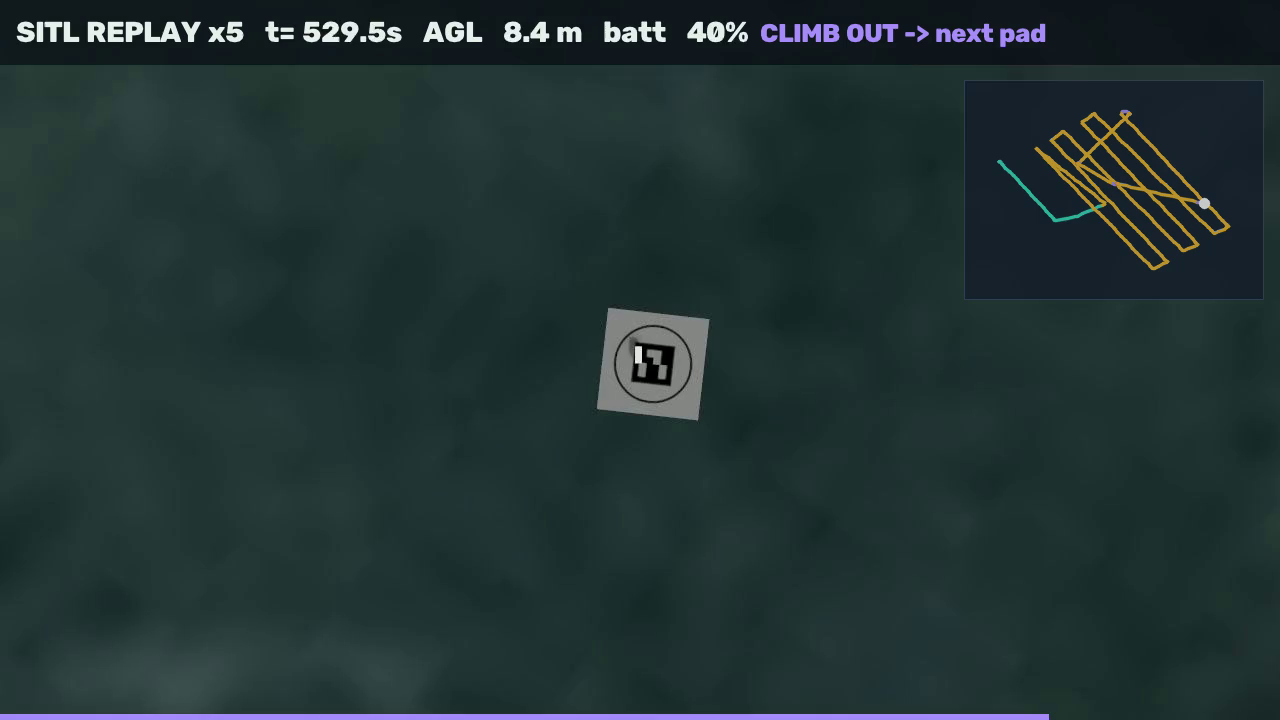
\includegraphics[width=0.78\textwidth,height=\textheight]{report_figures/sitl_mission_replay.png}
\caption{Simulation replay of a full four-egg mission. The main image is
the aircraft's own nadir camera over a pad at 8.4 m; the overlay carries
mission time, AGL, battery and phase, and the inset shows the flown
track --- the transit corridor in green and the completed survey sweep
in orange. Ground truth from the simulator is used only for the
post-flight audit, never for planning.}
\end{figure}

\hypertarget{b.2-real-flights-kmutnb-practice-field-standing-in-for-kmitl}{%
\subsection{B.2 Real flights (KMUTNB practice field, standing in for
KMITL)}\label{b.2-real-flights-kmutnb-practice-field-standing-in-for-kmitl}}

\begin{longtable}[]{@{}
  >{\raggedright\arraybackslash}p{(\columnwidth - 6\tabcolsep) * \real{0.1200}}
  >{\raggedright\arraybackslash}p{(\columnwidth - 6\tabcolsep) * \real{0.1200}}
  >{\raggedright\arraybackslash}p{(\columnwidth - 6\tabcolsep) * \real{0.2500}}
  >{\raggedright\arraybackslash}p{(\columnwidth - 6\tabcolsep) * \real{0.5100}}@{}}
\toprule\noalign{}
\begin{minipage}[b]{\linewidth}\raggedright
Date / time
\end{minipage} & \begin{minipage}[b]{\linewidth}\raggedright
Duration
\end{minipage} & \begin{minipage}[b]{\linewidth}\raggedright
What was flown
\end{minipage} & \begin{minipage}[b]{\linewidth}\raggedright
Outcome
\end{minipage} \\
\midrule\noalign{}
\endhead
\bottomrule\noalign{}
\endlastfoot
20 Aug & 3 flights & First outdoor autonomy: transit + sweep &
\textbf{Found:} every waypoint was sent with an undefined yaw, so PX4
turned the nose at each one --- \textbf{867° of yaw in 122 s}, and the
body-fixed camera spun with it (1 of 457 frames decoded).
\textbf{Found:} the GPS height reference inflated the reported AGL and
returned a flight that was tracking transit to 1.7 m. Both fixed (single
sweep heading; barometric height reference) \\
21 Aug & bench, props off & \textbf{Pilot-takeover drill} on the real
flight controller and companion & Stand-down at the 1 s debounce
verified; no companion command can fight the pilot \\
24 Aug & 2 flights (from the FC's own log) & Take-off gate investigation
& \textbf{Found:} PX4 leaves AUTO\_TAKEOFF as soon as it is within
\texttt{NAV\_MC\_ALT\_RAD} of the target, levelling off 0.8 m low and
aborting an otherwise perfect mission at take-off \\
26 Aug & 3 flights & Sweep with the new envelope & \textbf{Found:} PX4's
own vertical fence returned a correctly-flying aircraft (its home
altitude had walked 14 m in 93 s), the mission did not notice, and its
next waypoint reached the aircraft while the return was \textbf{0.46 m
from touchdown}. \textbf{Found:} 2,788 frames, \textbf{0 decodes}, with
a pad plainly in view --- the white pad was clipped at 255 by an
exposure metered on grass. Both fixed (FC-failsafe stand-down,
home-altitude latch, highlight-priority exposure); ids decoded in the
air later the same day \\
27 Aug 12:44 & 5 min 56 s & \textbf{Full 7-leg survey}, 6,044 frames &
\textbf{5 of 6 pads decoded and confirmed} (votes 13--14, confidence
0.95). The sixth pad is \textbf{printed with marker id 0} and was being
filtered out --- the reason the valid set is now 0--6 \\
27 Aug 14:13 & --- & Survey + serve & Confirmed all three of its
assigned ids at \textbf{t = 52 s} and kept sweeping to leg 5 of 7. The
sweep now stops as soon as every id the flight owes is confirmed \\
27 Aug 14:51 & --- & First delivery attempt & \textbf{First real egg
placed on a pad: 0.14 m from centre}, released after touchdown. Exposed
a false failsafe on our own landing, fixed the same day \\
\textbf{27 Aug 15:25} & \textbf{4 min 12 s} & \textbf{Complete mission,
end to end} & Transit ingress \textbf{3/3} → survey found 5 pads in
\textasciitilde20 s → early stop on the assigned ids → \textbf{land-ON
pad 1, release; land-ON pad 4, release} → egress → landed \textbf{0.7 m}
from the launch point → disarm. \textbf{2/2 delivered.} Aircraft health:
14--16 satellites, horizontal accuracy ≤ 2 m, companion CPU 41 \%, hover
throttle 0.59--0.64, allocator never saturated, and the home-altitude
latch held silent through five home rewrites \\
\end{longtable}

\hypertarget{b.3-what-the-flight-record-establishes}{%
\subsection{B.3 What the flight record
establishes}\label{b.3-what-the-flight-record-establishes}}

\begin{itemize}
\tightlist
\item
  The \textbf{full sequence works on real hardware}: gate, transit,
  survey, registry, id-verified descent, land-ON, touchdown-gated
  release, egress, landing, disarm.
\item
  \textbf{Release accuracy on the real aircraft (0.14 m)} is consistent
  with the simulated 0.09--0.30 m band, so the terminal controller is
  not simulator-flattered.
\item
  Every safety layer added since 20 August has been \textbf{exercised in
  flight}, not only in tests: pilot takeover, FC-failsafe stand-down,
  the home-altitude latch, the early-stop sweep, and the release
  idempotence.
\item
  The \textbf{remaining unknown is endurance}, not capability (§3.2,
  Appendix C).
\end{itemize}

\begin{center}\rule{0.5\linewidth}{0.5pt}\end{center}

\hypertarget{appendix-c-open-items-and-risk-register}{%
\section{Appendix C --- Open items and risk
register}\label{appendix-c-open-items-and-risk-register}}

Stated in the order they matter on competition day.

\begin{longtable}[]{@{}
  >{\raggedright\arraybackslash}p{(\columnwidth - 4\tabcolsep) * \real{0.0400}}
  >{\raggedright\arraybackslash}p{(\columnwidth - 4\tabcolsep) * \real{0.2100}}
  >{\raggedright\arraybackslash}p{(\columnwidth - 4\tabcolsep) * \real{0.7500}}@{}}
\toprule\noalign{}
\begin{minipage}[b]{\linewidth}\raggedright
\#
\end{minipage} & \begin{minipage}[b]{\linewidth}\raggedright
Item
\end{minipage} & \begin{minipage}[b]{\linewidth}\raggedright
Status and mitigation
\end{minipage} \\
\midrule\noalign{}
\endhead
\bottomrule\noalign{}
\endlastfoot
1 & \textbf{Battery endurance vs the KMITL plan} & The indicated gauge
reaches the 15 \% return floor at roughly minute 8.5--10; the plan needs
10--13 minutes. \textbf{Mitigation, all implemented:} per-delivery
time-and-battery gate (gives up eggs, not the aircraft), planned 30 \%
egress through the scored corridor, second charged pack, automatic
recovery flight from the unfired latches. \textbf{Action:} record the
mAh returned by the charger after every flight --- it is the one
measurement that closes the question \\
2 & \textbf{The 28 Aug briefing changes are unflown} & 30 m ceiling, new
corridor P2′/P3′, cut search area, 20 m survey with 10.5 m decode
visits, 25 m failsafe RTL. The \textbf{13:00--18:00 trial slot is the
only test} before scoring \\
3 & \textbf{Committee coordinates not published} & Our corridor and
no-fly polygons are georeferenced from briefing photographs to
\textbf{±5 m}. Committee-published coordinates replace ours in both the
flight configuration and the ground station, same digits in both \\
4 & \textbf{Where the pads are placed} & The flown search area is cut at
E 110 m, west of the main building. \textbf{Pads placed east of the
building would not be searched.} Question to ask the committee before
the scored flights; routing around the building box is a day-2 change \\
5 & \textbf{RC-loss drill} & The parameters are pinned and read back,
but the net itself has never been exercised in the air. The diagnosis of
an earlier ``no pulses'' indication is closed (a held kill switch, not
the link) \\
6 & \textbf{CG record and structural margin} & Not formally documented
(§3.1). The aircraft is trimmed by flight behaviour; the cargo boxes are
heavier than the dummies in the weighed figure, so it is re-weighed with
real cargo at the field \\
7 & \textbf{Motor-map regression} & The motor map was once found reading
zero with no identified cause. It is re-read from the board before every
field day rather than trusted \\
8 & \textbf{Marker id 0 in the field configuration} & The flight
detector accepts ids 0--6 (correct). The \texttt{marker.valid\_ids} list
in the field configuration still reads 1--6; it is consumed only by the
simulator's pad spawner, so it cannot affect a real flight, but it
should be widened for consistency \\
9 & \textbf{Sim-only descent detail} & The per-rung descent ladder
writes the manual-mode descent parameter rather than its AUTO twin; the
effective pad approach is the pinned 0.4 m/s that every validated
landing has flown. Do not ``unpin'' it before the competition \\
\end{longtable}

\begin{center}\rule{0.5\linewidth}{0.5pt}\end{center}

\emph{Report structured to AAVC 2026 Rules \& Regulations V1.3, Appendix
A, as amended by the 24 July and 28 August 2026 event briefings. The
flight system is deterministic, classical-CV and offline: no machine
learning in the flight loop, no cloud, and no network --- network use is
an automatic disqualification. Supporting documents in this repository:
\texttt{docs/RULES\_AAVC2026.md} (rules digest), \texttt{docs/FLIGHT.md}
(field procedure), \texttt{docs/SERVO\_AUX\_MAPPING.md} (payload
wiring), \texttt{docs/evidence/} (flight and bench evidence).}

\end{document}
